\documentclass{article}
\usepackage[utf8]{inputenc}
\usepackage{hyperref}
\hypersetup{
    colorlinks=true,
    linkcolor=blue,
    filecolor=blue,      
    urlcolor=blue,
}
\usepackage[a4paper,top=2cm,bottom=2.5cm,left=2cm,right=2cm,marginparwidth=1.75cm]{geometry}
\usepackage{float}
\usepackage{forest}
\usepackage{graphicx}
\graphicspath{ {images/} }
\title{\textbf{\underline{Attendo Design Document}}}
\author{
\textbf{Team - 13}\\
Angad Kambli, 19114041\\ 
Ayush Gupta, 191114017 \\ 
Chirag Wadhwa, 19114023 \\ 
Devanshu Chowdhury, 19114027 \\ 
Shubham Bansode, 19114019 }
\date{}
\begin{document}

\maketitle

\begin{abstract}
    \textbf{Attendo} is developed by us as an app to streamline marking attendance in classroom settings. It is developed using the \textbf{Flutter} framework and it makes use of \textbf{Network Service Discovery} and \textbf{Socket Programming} for the networking part and \textbf{Firebase} for backend. It aims at making the attendance process quick and easy for both the teachers and the students. The following document will give a thorough description of the methods used in the implementation of the app, the tech stack and the thinking behind selecting it, some design decisions and clever approaches applied by us and the UML diagrams. The code is hosted on GitHub and can be accessed \href{https://github.com/Attendo-App/Attendo}{here}.
\end{abstract}
\tableofcontents
\newpage

\section{Introduction}
\subsection{Problem Statement}
Classical methods used in classrooms to take attendance are cumbersome and time taking. Also, calling out names also gives a rise to the issue of not being able to maintain the sanctity of records due to students marking proxies. Also, it is disadvantageous for both professors and students with respect to availability of data. For the professor, it is a pain to physically comb through the records to check whether a certain student fulfills the minimum criteria. For the student, he has to keep a record of how many classes he has attended and if he doesn't, there are chances he would never understand his attendance is dangerously low before it's too late. With the availability of mobile devices, it is high time that we start making use of it for taking attendance.
\subsection{The Solution}
With \textbf{Attendo}, we bring a solution to all these qualms. With a simple and well-designed UI, it can be easily introduced in classroom settings. It makes sure every device can mark attendance only once thus guaranteeing the sanctity of records. The professor can easily check the attendance percentage of his students and can also check every lecture's record which might prove useful in detecting patterns in attendance statistics. With the records easily accessible at any time, a student can correct his habits well in time if his attendance percentage is low.

\section{Division of labour}
While all the team members were involved in the brainstorming for deciding the app's flow and implementation, there was a clear division of labour with regards to the domains a certain person would be responsible for. Following are the contributions of various members :
\begin{enumerate}
    \item \textbf{Angad Kambli, 19114041 :} Initialization of project, implementation of socket programming and network service discovery, coding the login and registration screen UI and other UI fixes, maintaining the GitHub repository(reviewing PRs, solving merge conflicts and so on), the course image solution, designing the icon and other minor fixes.
    \item \textbf{Ayush Gupta, 191114017 : } Setting up Firebase in the app, setting up authentication logic for the user, writing database queries for read and writes, writing controller functions to clean data recieved from database and add minor functionality in registration pages.
    \item \textbf{Chirag Wadhwa, 19114023 : } Implementing the flow of taking and marking attendance, implementing the logic to prevent multiple attendance markings from the same device, Major final changes to bring all the implementation together and to remove all hard coded values and replace them with database query calls, final bug fixes and testing.
    \item \textbf{Devanshu Chowdhury, 19114027 : } Designing the UI for the App. Coding most of the Screens including the Dialogue Boxes showing successful and failed errors , designing hard-coded List Views and minor visual changes to the UI to make the design more attractive and comprehensible.
    \item \textbf{Shubham Bansode, 19114019 : }  Writing database queries for read and writes, writing controller functions to clean data recieved from database, final screenshots.
\end{enumerate}

\section{Use Case Diagram}
\begin{figure}[H]
    \centering
    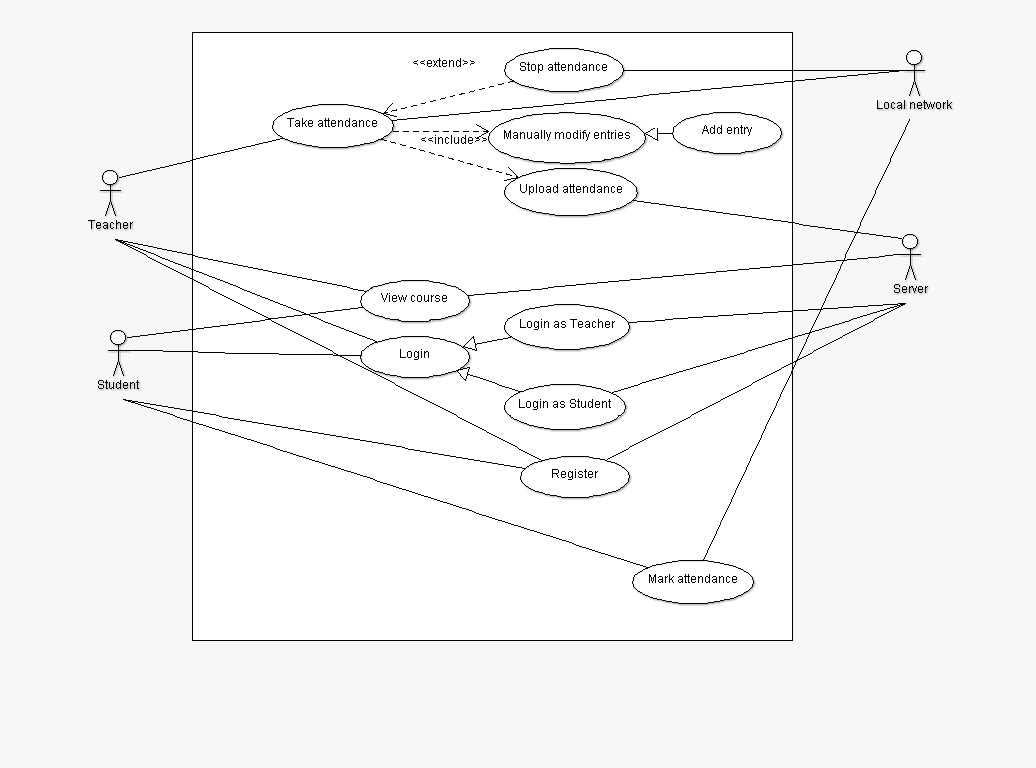
\includegraphics[width=0.95\textwidth]{UseCase.jpeg}
    \caption{Use Case Diagram}
    \label{fig:UseCase}
\end{figure}

\textbf{Use Case 1 :} Register \\
\textbf{Actor :} Student, Professor \\
\textbf{Pre-conditions :} Is not already registered\\
\textbf{Basic Flow :}
\begin{itemize}
    \item Scenario 1 : Mainline Sequence
        \begin{enumerate}
            \item Student/Professor : Enter credentials and tap on the register button.
            \item AuthService : Pass the credentials to the database for checking validity.
            \item  Database:  Check credentials for validity.        
\end{enumerate}
   \item Scenario 2: At Step 4 of Mainline Sequence 
        \begin{enumerate}
            \setcounter{enumi}{3}
            \item Database: return the user id if credentials are valid.
	\item AuthService: display successful dialog box. 
        \end{enumerate}  
    \item Scenario 3: At Step 4 of Mainline Sequence 
        \begin{enumerate}
            \setcounter{enumi}{3}
            \item Database: return null if credentials not valid
	\item AuthService: print error message. 
        \end{enumerate}  
\end{itemize}
\textbf{Post-Conditions:} Is registered\\ \\
\textbf{Use Case 2:} Login\\
\textbf{Actor :} Student, Professor \\
\textbf{Pre-conditions :}Is a registered user\\
\textbf{Basic Flow :} 
\begin{itemize}
    \item Scenario 1: Mainline Sequence
\begin{enumerate}
\item Student/Professor : This use case starts when a user wishes to log in into the System. 
\item System : requests that the user enter his/her Login Information i.e Email ID and Password. 
\item Student/Professor : Insert his/her Email and Password. 	
\item Controller: The System then validates the entered Email ID and password.
\item Controller : Confirm Log in
\end{enumerate}
	\item Scenario 2: At Step 4
	    \begin{enumerate}
	        \setcounter{enumi}{3}
		    \item System : Show error
	    \end{enumerate}
		
\end{itemize}
\textbf{Post-Conditions:} Is logged in\\ \\
\textbf{Use Case 3 :} Mark Attendance \\
\textbf{Actor :} Student,Local Network\\
\textbf{Pre-conditions :}  Is logged in as a student and is also registered in course\\
\textbf{Basic Flow :}
\begin{itemize}
    \item Scenario 1 : Mainline Sequence
        \begin{enumerate}
            \item Student : Click Mark Attendance Button
	\item Local Network: Discover service,get ip and port of server
	\item Local Network: Connect to server using ip and port
	\item Local Network: Communicate enrollment number to server
        \end{enumerate}
   \item Scenario 2 : At Step 5 of Mainline Sequence
        \begin{enumerate}
	\setcounter{enumi}{4}
            \item Local Network: Send “OK” message from server to Student
	\item System: Displays attendance success dialogue
        \end{enumerate}
 \item Scenario 3: At Step 5 of Mainline Sequence
       \begin{enumerate}
	\setcounter{enumi}{4}
	\item Local Network: Send “Error” message from server to Student
	\item System: Displays attendance failure dialogue
     \end{enumerate}
\end{itemize}
\textbf{Post-Conditions:} If the IP address is unique,attendance is marked for the selected course.\\ \\
\textbf{Use Case 5 : }View Course\\
\textbf{Actor : }Student, Professor\\
\textbf{Preconditions : }Is logged in\\
\textbf{Basic Flow: } 
\begin{itemize}
    \item Scenario 1 : Mainline Sequence
        \begin{enumerate}
            \item Student/Professor : Select Course
            \item System: Request Course Details
            \item  Database:  Return Course Details
\item System : Format and Display details accordingly.        
\end{enumerate}
\end{itemize}
\textbf{Post-Conditions: }User can view course details for the selected course\\



\section{Class Diagram}
\begin{figure}[H]
    \centering
    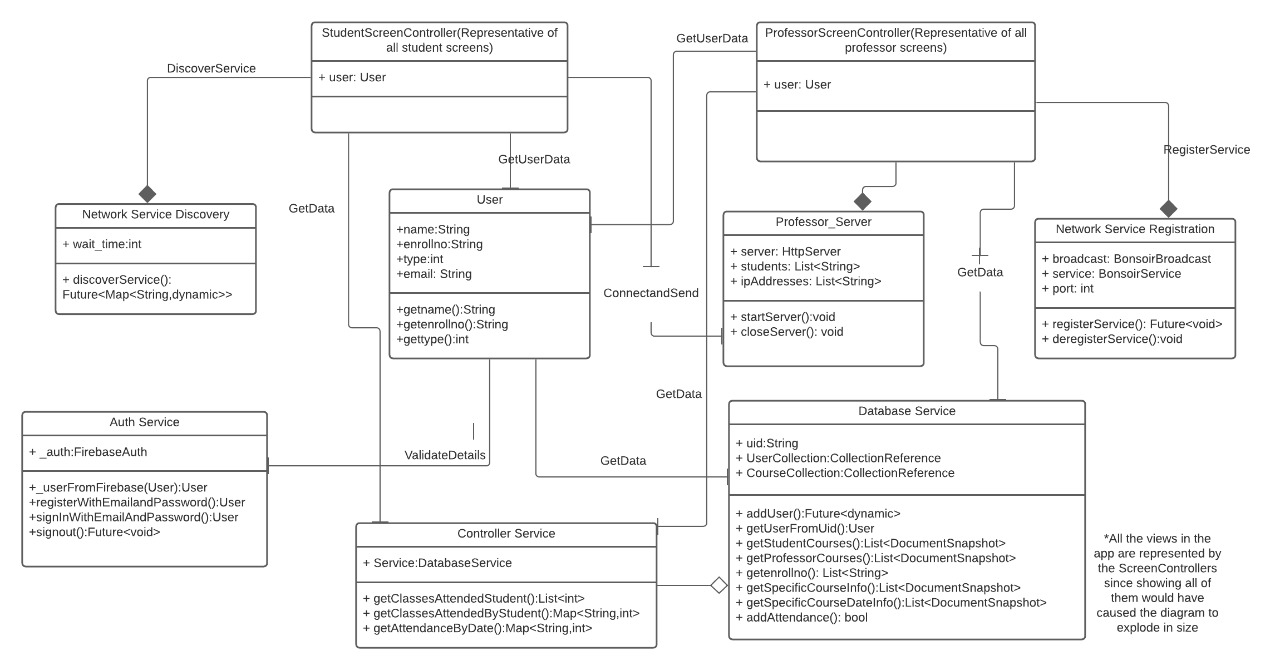
\includegraphics[width=0.95\textwidth]{ClassDiagram.jpeg}
    \caption{Class Diagram}
    \label{fig:ClassDiagram}
\end{figure}

\section{Sequence Diagram} 
\subsection{Mark Attendance Use Case}
\begin{figure}[H]
    \centering
    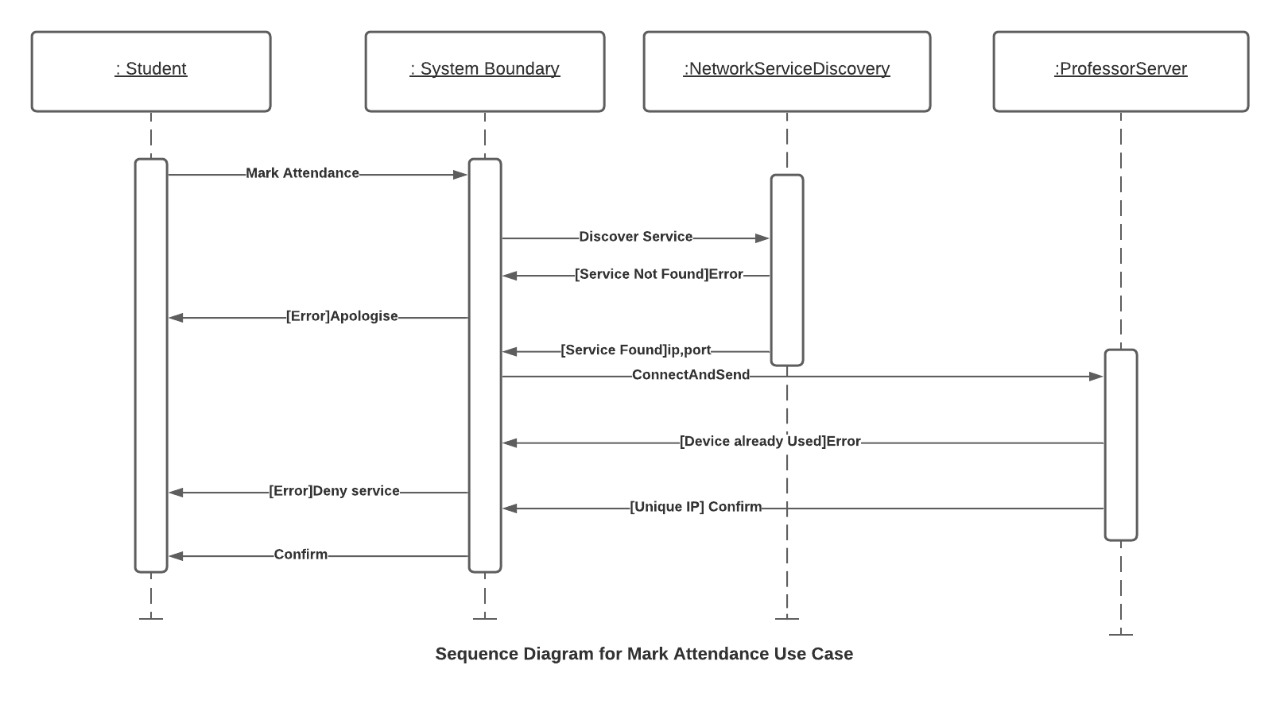
\includegraphics[width=0.95\textwidth]{MarkAttendance.jpeg}
    \caption{}
    \label{fig:MarkAttendace}
\end{figure}
\subsection{Take Attendance Use Case}
\begin{figure}[H]
    \centering
    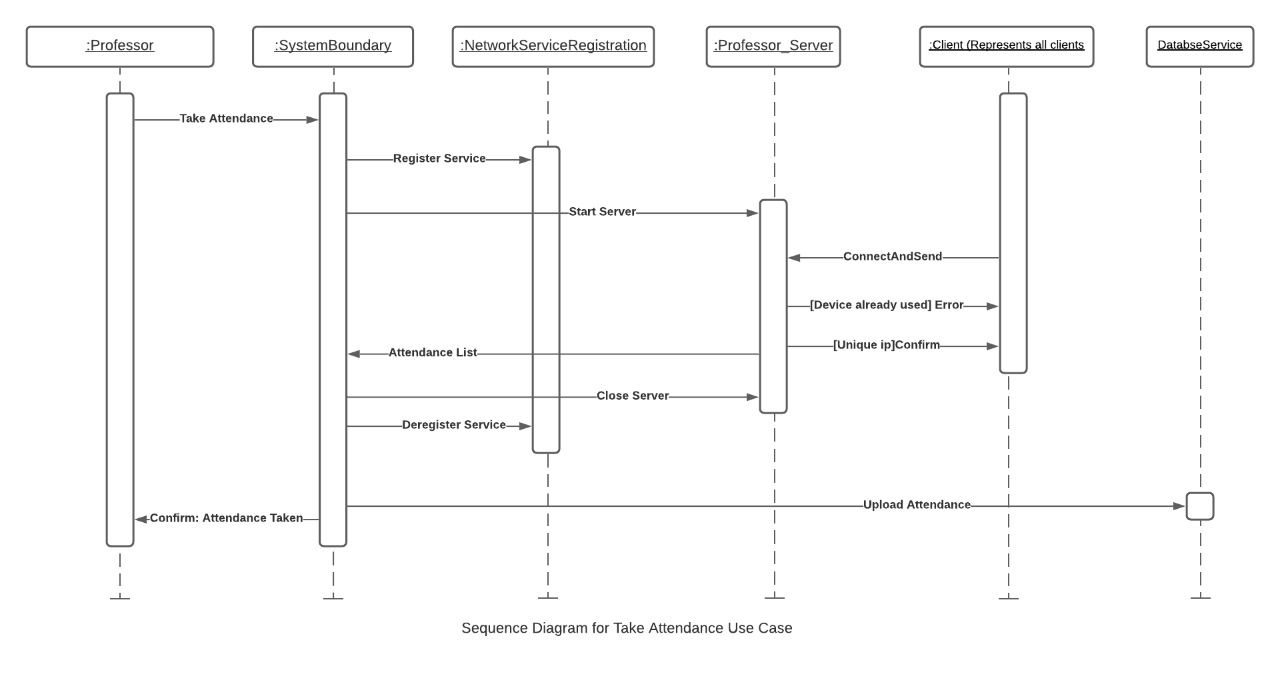
\includegraphics[width=0.95\textwidth]{TakeAttendace.jpeg}
    \caption{}
    \label{fig:TakeAttendace}
\end{figure}
\subsection{Login Use Case}
\begin{figure}[H]
    \centering
    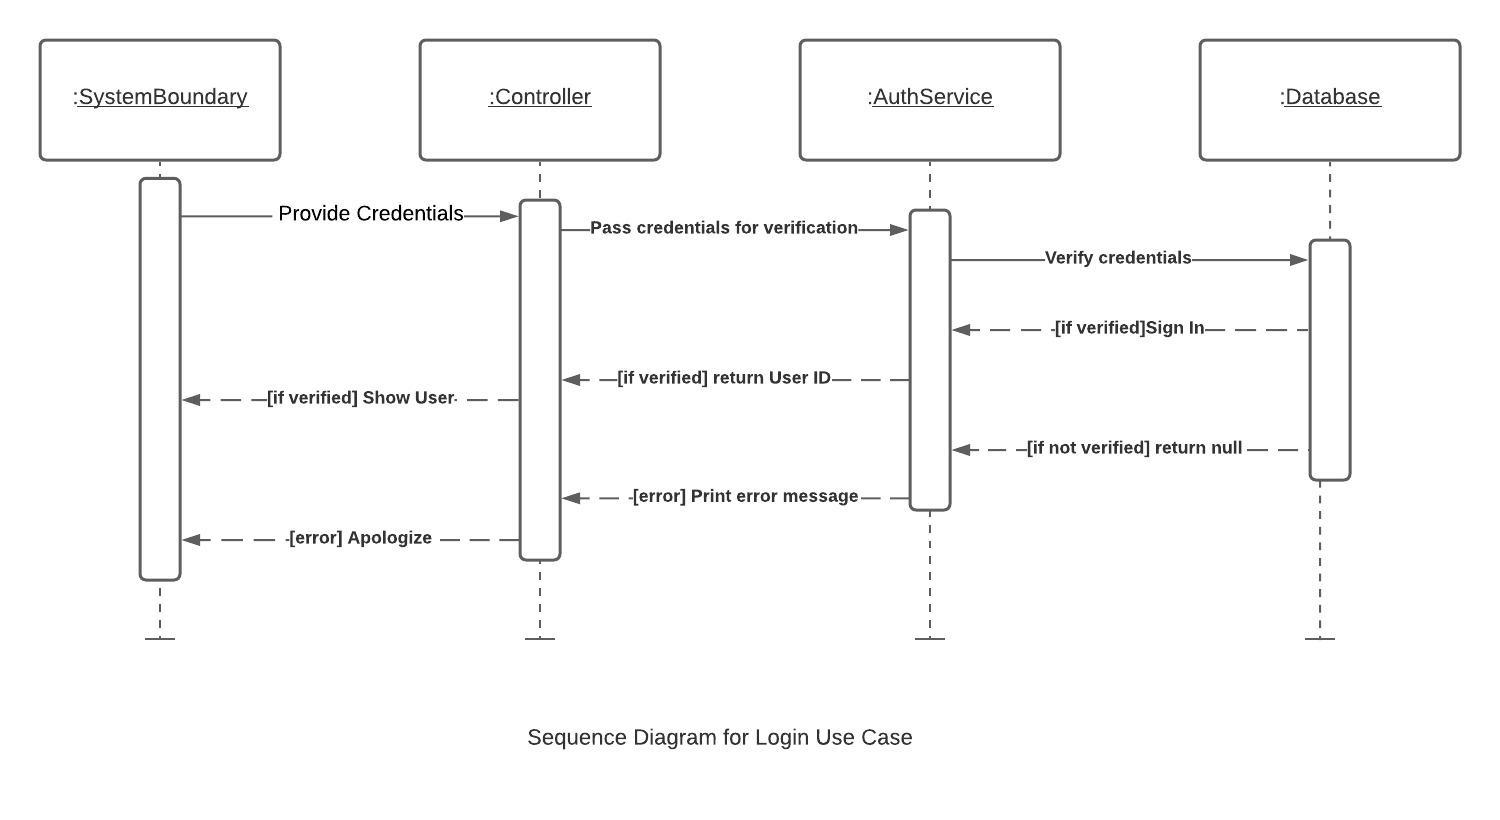
\includegraphics[width=0.95\textwidth]{login sequence diagram.jpeg}
    \caption{}
    \label{fig:Login}
\end{figure}
\subsection{Register Use Case}
\begin{figure}[H]
    \centering
    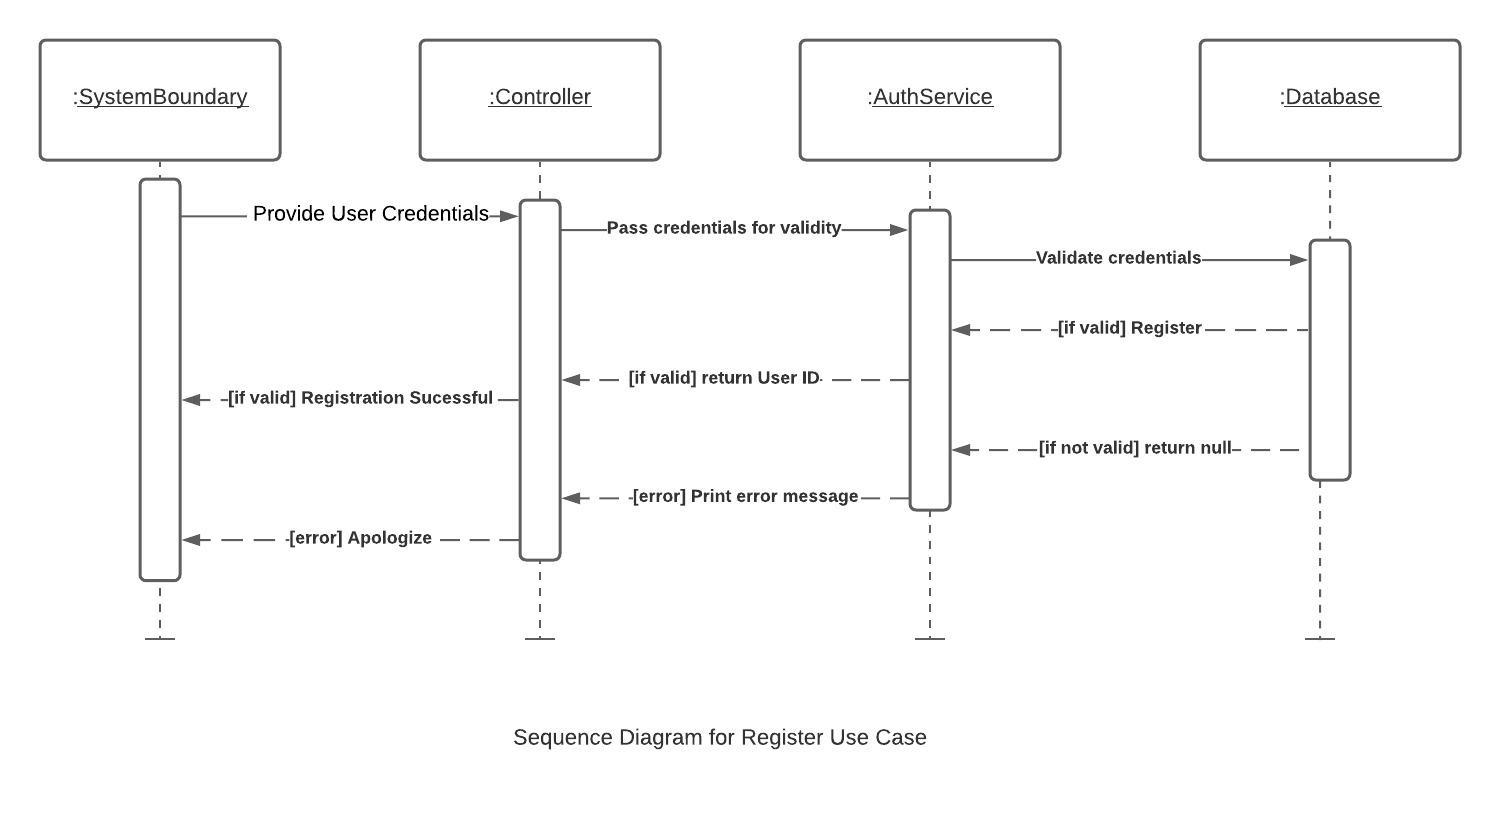
\includegraphics[width=0.95\textwidth]{register sequence diagram.jpeg}
    \caption{}
    \label{fig:register}
\end{figure}
\subsection{View Course Use Case}
\begin{figure}[H]
    \centering
    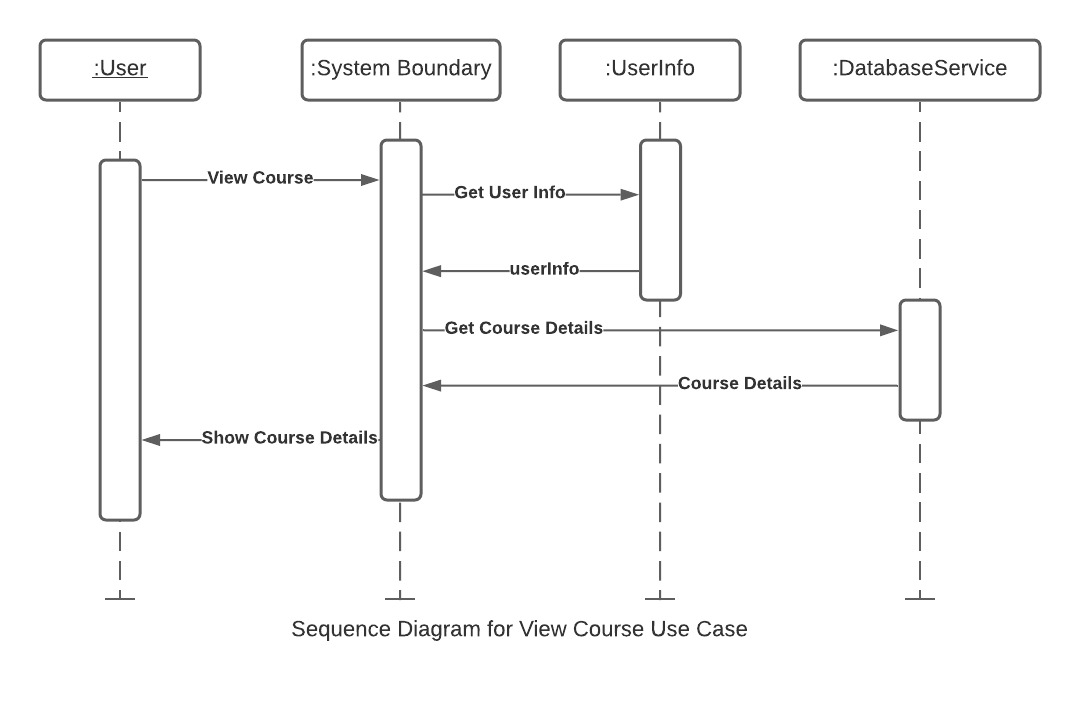
\includegraphics[width=0.95\textwidth]{ViewCourse.jpeg}
    \caption{}
    \label{fig:ViewCourse}
\end{figure}

\section{Tech stack}
The different frameworks, technologies and libraries used for the implementation will be discussed in the following subsections.
\subsection{Flutter}
Flutter is a framework developed by Google mainly for increasing the productivity of Mobile development workflow but has also been extended for web app development. Here, we had the choice of either going with Flutter or going the route of native Android development. Th motivation behind selecting Flutter was some of the added benefits that Flutter gives which includes but are not limited to :
\begin{itemize}
    \item Flutter can build for both iOS and Android with very less extra coding. This is in stark contrast to native Android or iOS development which requires a lot of redundant coding. However, for now, we have built the app only for Android but a build for iOS wouldn't be a huge undertaking in case the app needs to be actually used in classroom situations.
    \item Flutter provides the hot reload feature which really speeds up development. Native Android coding requires us to reinstall the app to check for new changes which can become a real pain once the app increases in size.
    \item Flutter unifies the UI design and the logic which is a huge relief from native Android development's requirement for writing XML files for each screen.
    \item Last but not the least, Flutter provides some really good widgets that require little or no less customization before they look good.
\end{itemize}
\subsection{Firebase}
Firebase was used as the backend for the app. This was a no-brainer choice since the backend requirements of the app aren't very complex and Firebase provides an easy to setup interface. It was used by us for both Authentication and Database handling. Firebase provides two types of databases. The one we used is Cloud Firestore. It is a noSQL (JSON based) database. The app includes an API key which the app uses to communicate with Firebase.
\subsection{Bonsoir (Network Service Discovery)}
Bonsoir is an open source Flutter library that we used for Network Service Discovery. Network Service Discovery is used for registering the attendance service over the network from the professor side and is then used from the student side to get the host and port of the professor's phone. In native Android development, this would have been an in-built feature but since Flutter is coded in dart, we have to use libraries that further get ported to both Android and iOS.
\subsection{Socket Programming}
Socket programming was done using the TCP protocol. On professor's side, a server is created which the student side communicates through socket programming. 

\section{Architecture and the directory structure}
The architecture is loosely based on the \textbf{Model-View-Controller(MVC)}. We say loosely because the division of labour between the models, views and controllers that is usually expected wasn't followed as strictly by us. Some of controller workload is shared by the models and some by the views.
The views are in the screens since its a convention to call the views as screens in Flutter development. The file \emph{main.dart} is the entrypoint for the app and the flow of code starts from there itself. The directory structure is as follows :
\newline
\newline
\begin{forest}
  for tree={
    font=\ttfamily,
    grow'=0,
    child anchor=west,
    parent anchor=south,
    anchor=west,
    calign=first,
    edge path={
      \noexpand\path [draw, \forestoption{edge}]
      (!u.south west) +(7.5pt,0) |- node[fill,inner sep=1.25pt] {} (.child anchor)\forestoption{edge label};
    },
    before typesetting nodes={
      if n=1
        {insert before={[,phantom]}}
        {}
    },
    fit=band,
    before computing xy={l=15pt},
  }
[lib
  [models
    [all the model files]
  ]
  [controller
    [all the controller files]
  ]
  [screens
    [all the views or screens]
  ]
  [networking
    [socket-programming.dart]
    [network-service-discovery.dart]
  ]
  [main.dart (entrypoint)]
]
\end{forest}


\section{Implementation of networking}
The actual act of taking attendance is divided into two parts on both the professor and the student sides. The two parts are concerned with network service discovery(NSD) and socket programming respectively.
\\
Let's delve into the details of the professor's flow.
Once the professor taps on take attendance, first a service is registered on the network with the host and port and the service name using NSD. Next, a TCP server is started by the professor's phone and it starts listening for connections. Once a connection is recieved, it checks whether it is from an IP address that hasn't already marked attendance and adds the enrollment number to the attended list accordingly. Since this is happening on the local network, students can't fool the system by using a VPN. Also, by ensuring the same IP can't mark attendance twice, we make sure that the student can't mark attendance twice using the same device.
\\
On the student side, the phone searches for the service using nsd and gets the required host and port. It then connects to the service, sends the enrollment number and disconnects.
\\
The networking is done in TCP and NSD is implemented using a flutter library \emph{Bonsoir}.

\section{The Database Schema}
Firebase includes includes alternating JSON based documents and their collections in its database. The following is the Database Schema :
\newline
\newline
\hfill
\begin{forest}
  for tree={
    font=\ttfamily,
    grow'=0,
    child anchor=west,
    parent anchor=south,
    anchor=west,
    calign=first,
    edge path={
      \noexpand\path [draw, \forestoption{edge}]
      (!u.south west) +(7.5pt,0) |- node[fill,inner sep=1.25pt] {} (.child anchor)\forestoption{edge label};
    },
    before typesetting nodes={
      if n=1
        {insert before={[,phantom]}}
        {}
    },
    fit=band,
    before computing xy={l=15pt},
  }
  [Root Document
      [Courses Collection
            [Course Documents
                [Enrollment-numbers-list]
                [Course Code]
                [Course Name]
                [Professor Name]
                [Lectures Collection
                    [Lecture Documents
                        [List of enrollment numbers of attended students]
                        [Date]
                    ]
                ]
            ]
          ]
    [Users Collection
      [User Documents
        [Enrollment number]
        [Name]
        [User Type (Teacher/Student)]
        [User ID]
      ]
     ]
    ]
\end{forest}
\hfill

\section{Course Display Image Solution}
We had hard-coded the course display image for most of our development period. However, it is important to have a recognizable and good looking image associated with every course to improve the user experience. Now, to give the option for users to customize the display pictures for every course would be a major undertaking since it would involve storing each and every image which wouldn't be desirable since such storage requirements would hurt the scalability of the project.
\begin{figure}[h]
    \centering
    
\includegraphics[width=0.09\textwidth]{course-img1.png}
    
\includegraphics[width=0.09\textwidth]{course-img2.png}
    
\includegraphics[width=0.09\textwidth]{course-img3.png}
    
\includegraphics[width=0.09\textwidth]{course-img4.png}
    
\includegraphics[width=0.09\textwidth]{course-img5.png}
    
\includegraphics[width=0.09\textwidth]{course-img6.png}
    
\includegraphics[width=0.09\textwidth]{course-img7.png}
    
\includegraphics[width=0.09\textwidth]{course-img8.png}
    
\includegraphics[width=0.09\textwidth]{course-img9.png}
    
\includegraphics[width=0.09\textwidth]{course-img10.png}
    \caption{The Course Display icons}
    \label{fig:UseCase}
\end{figure}
\\Keeping this in mind, we created ten abstract, simple and snappy icons for different courses. While making it seemingly random to the user,the image is still chosen deterministically to ensure that it remains constant for any particular course. We decided to take the modulo of the number formed by the last two digits of the course code as the index that would select one icon out of the ten we made. 
\\This would make the home page much more vivid and also improve the User Experience since we tend to associate images and text and having that remembrance value always helps.

\section{Snapshots}
\begin{figure}[H]
    \centering
    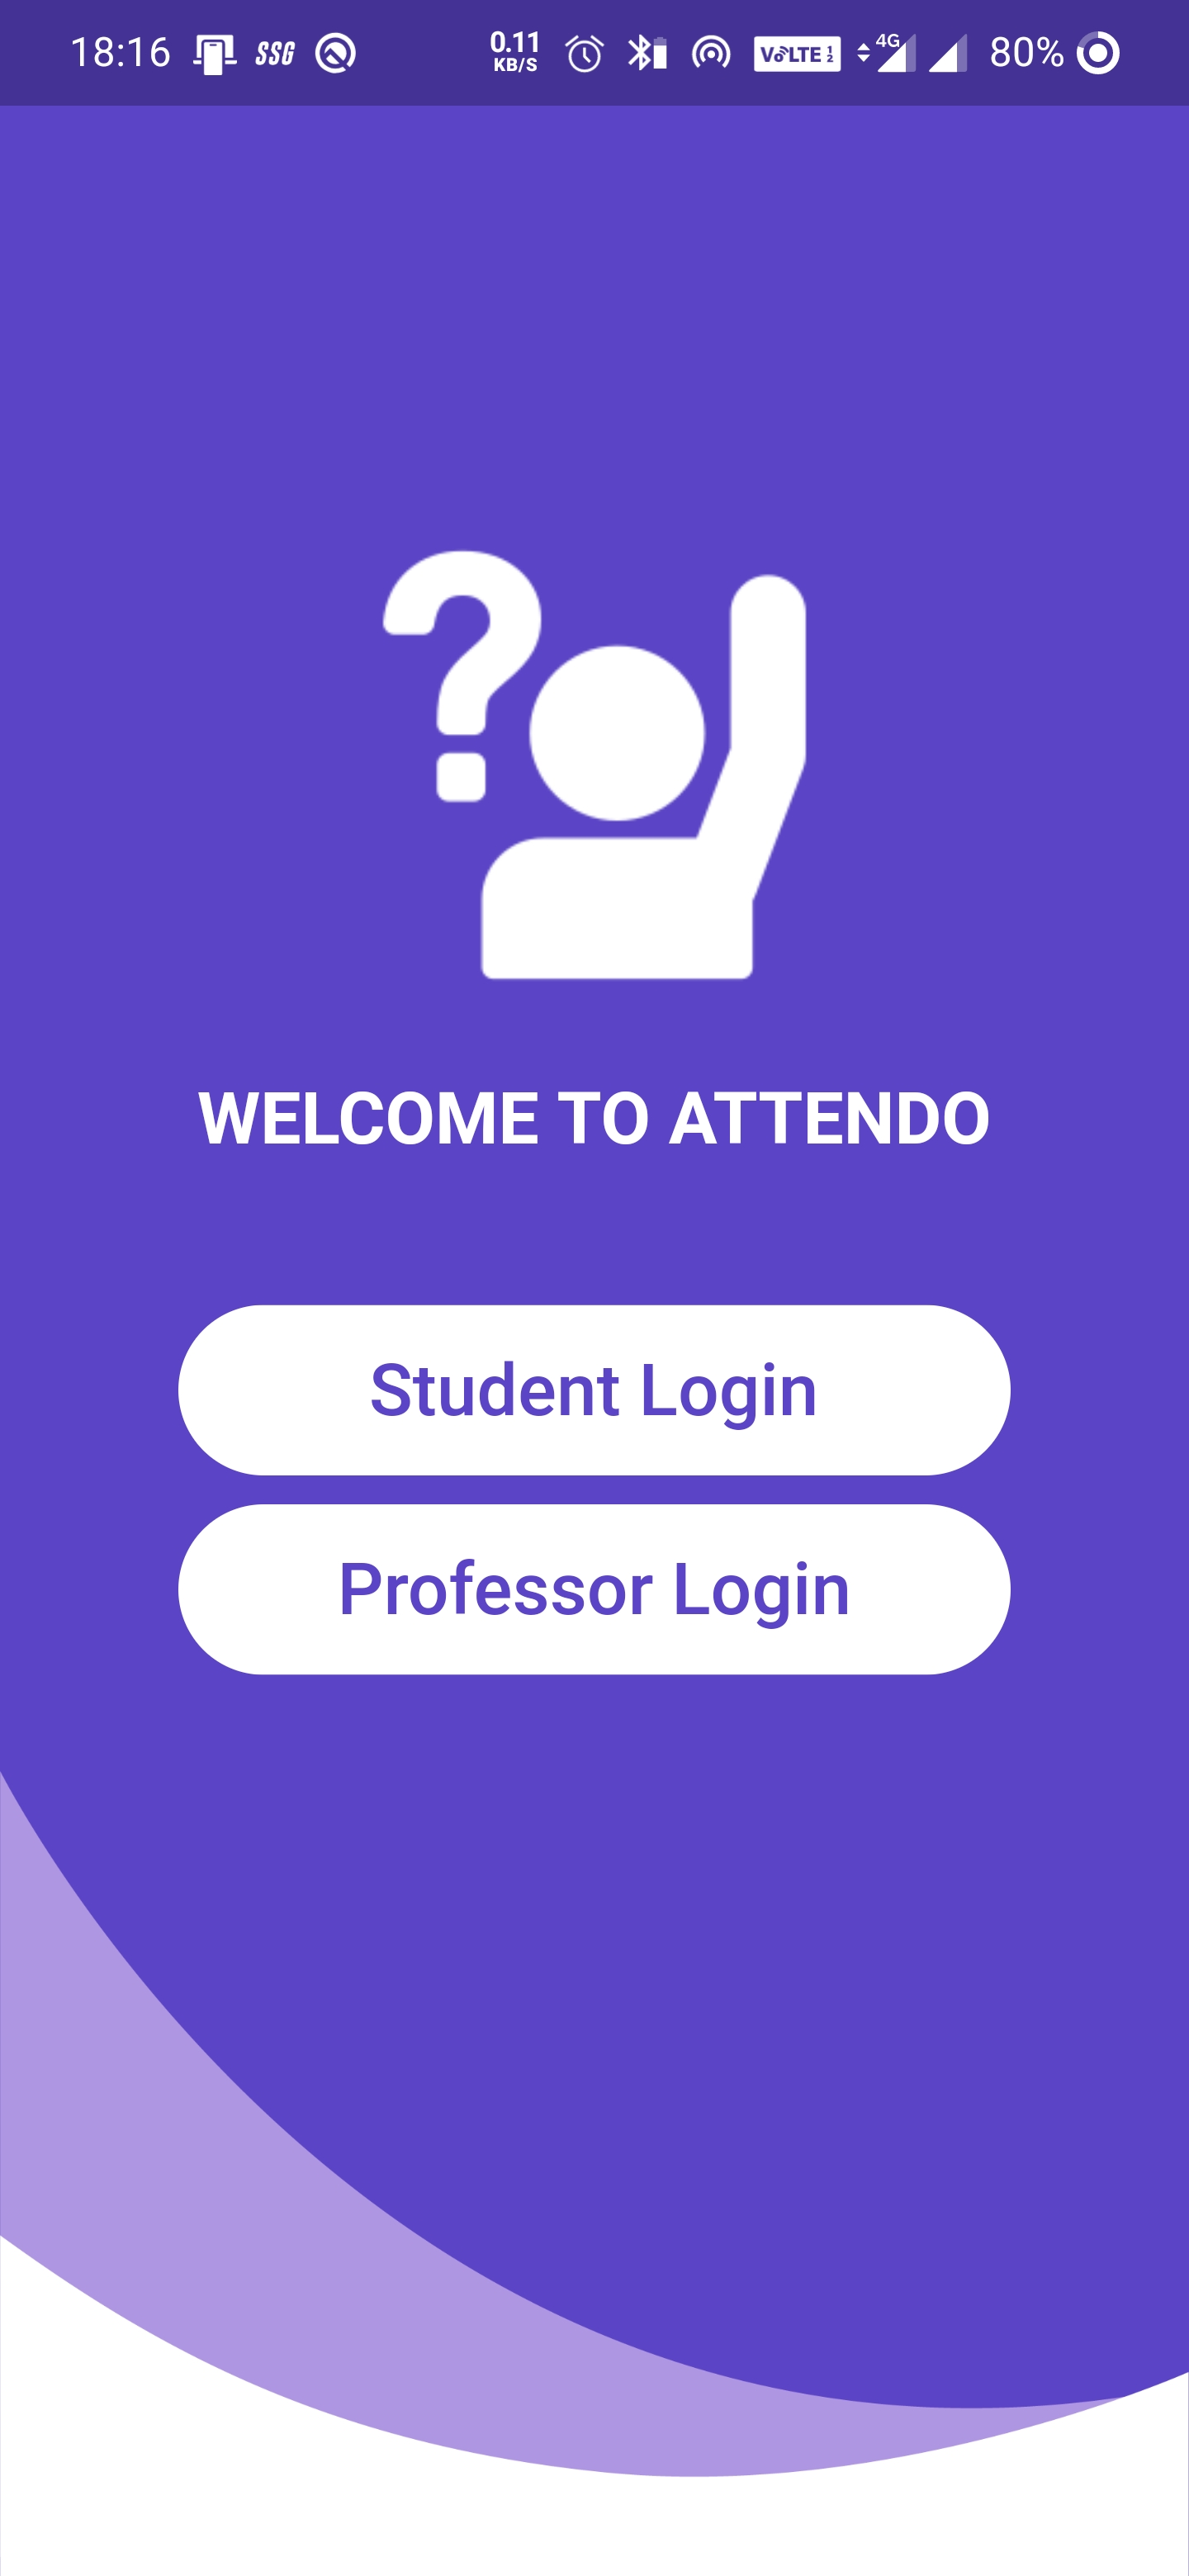
\includegraphics[width=0.50\textwidth]{HomeScreen[1].jpg}
    \caption{Auth Landing Screen}
    \label{fig:HomeScreen}
\end{figure}
\begin{figure}[H]
    \centering
    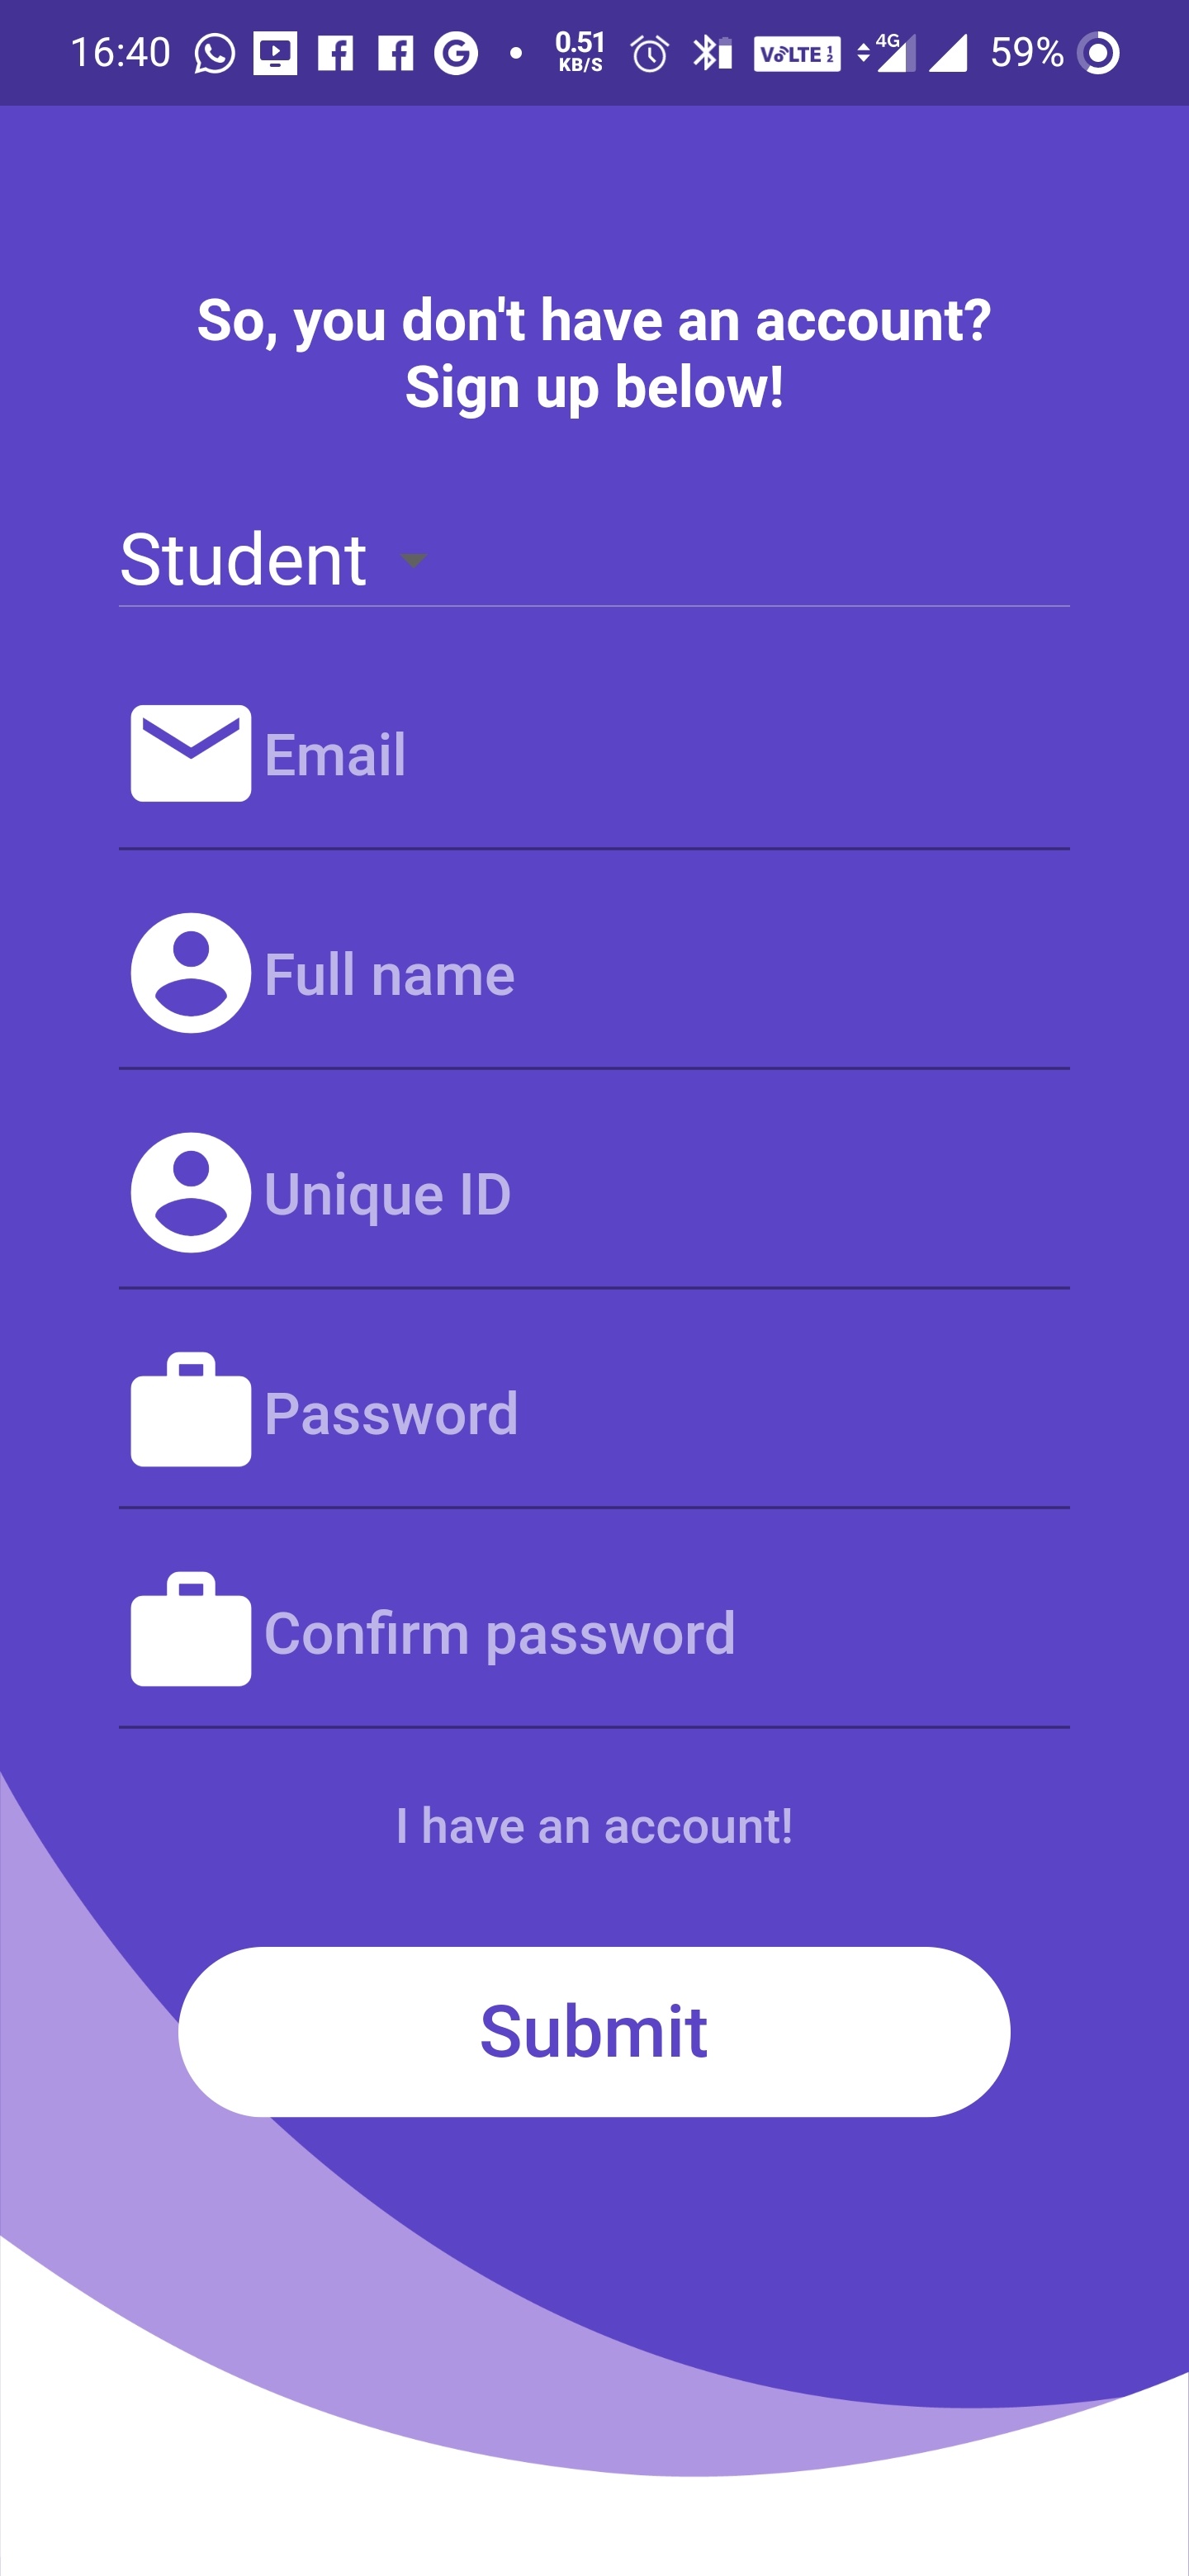
\includegraphics[width=0.40\textwidth]{Studentregisteration.jpg}
    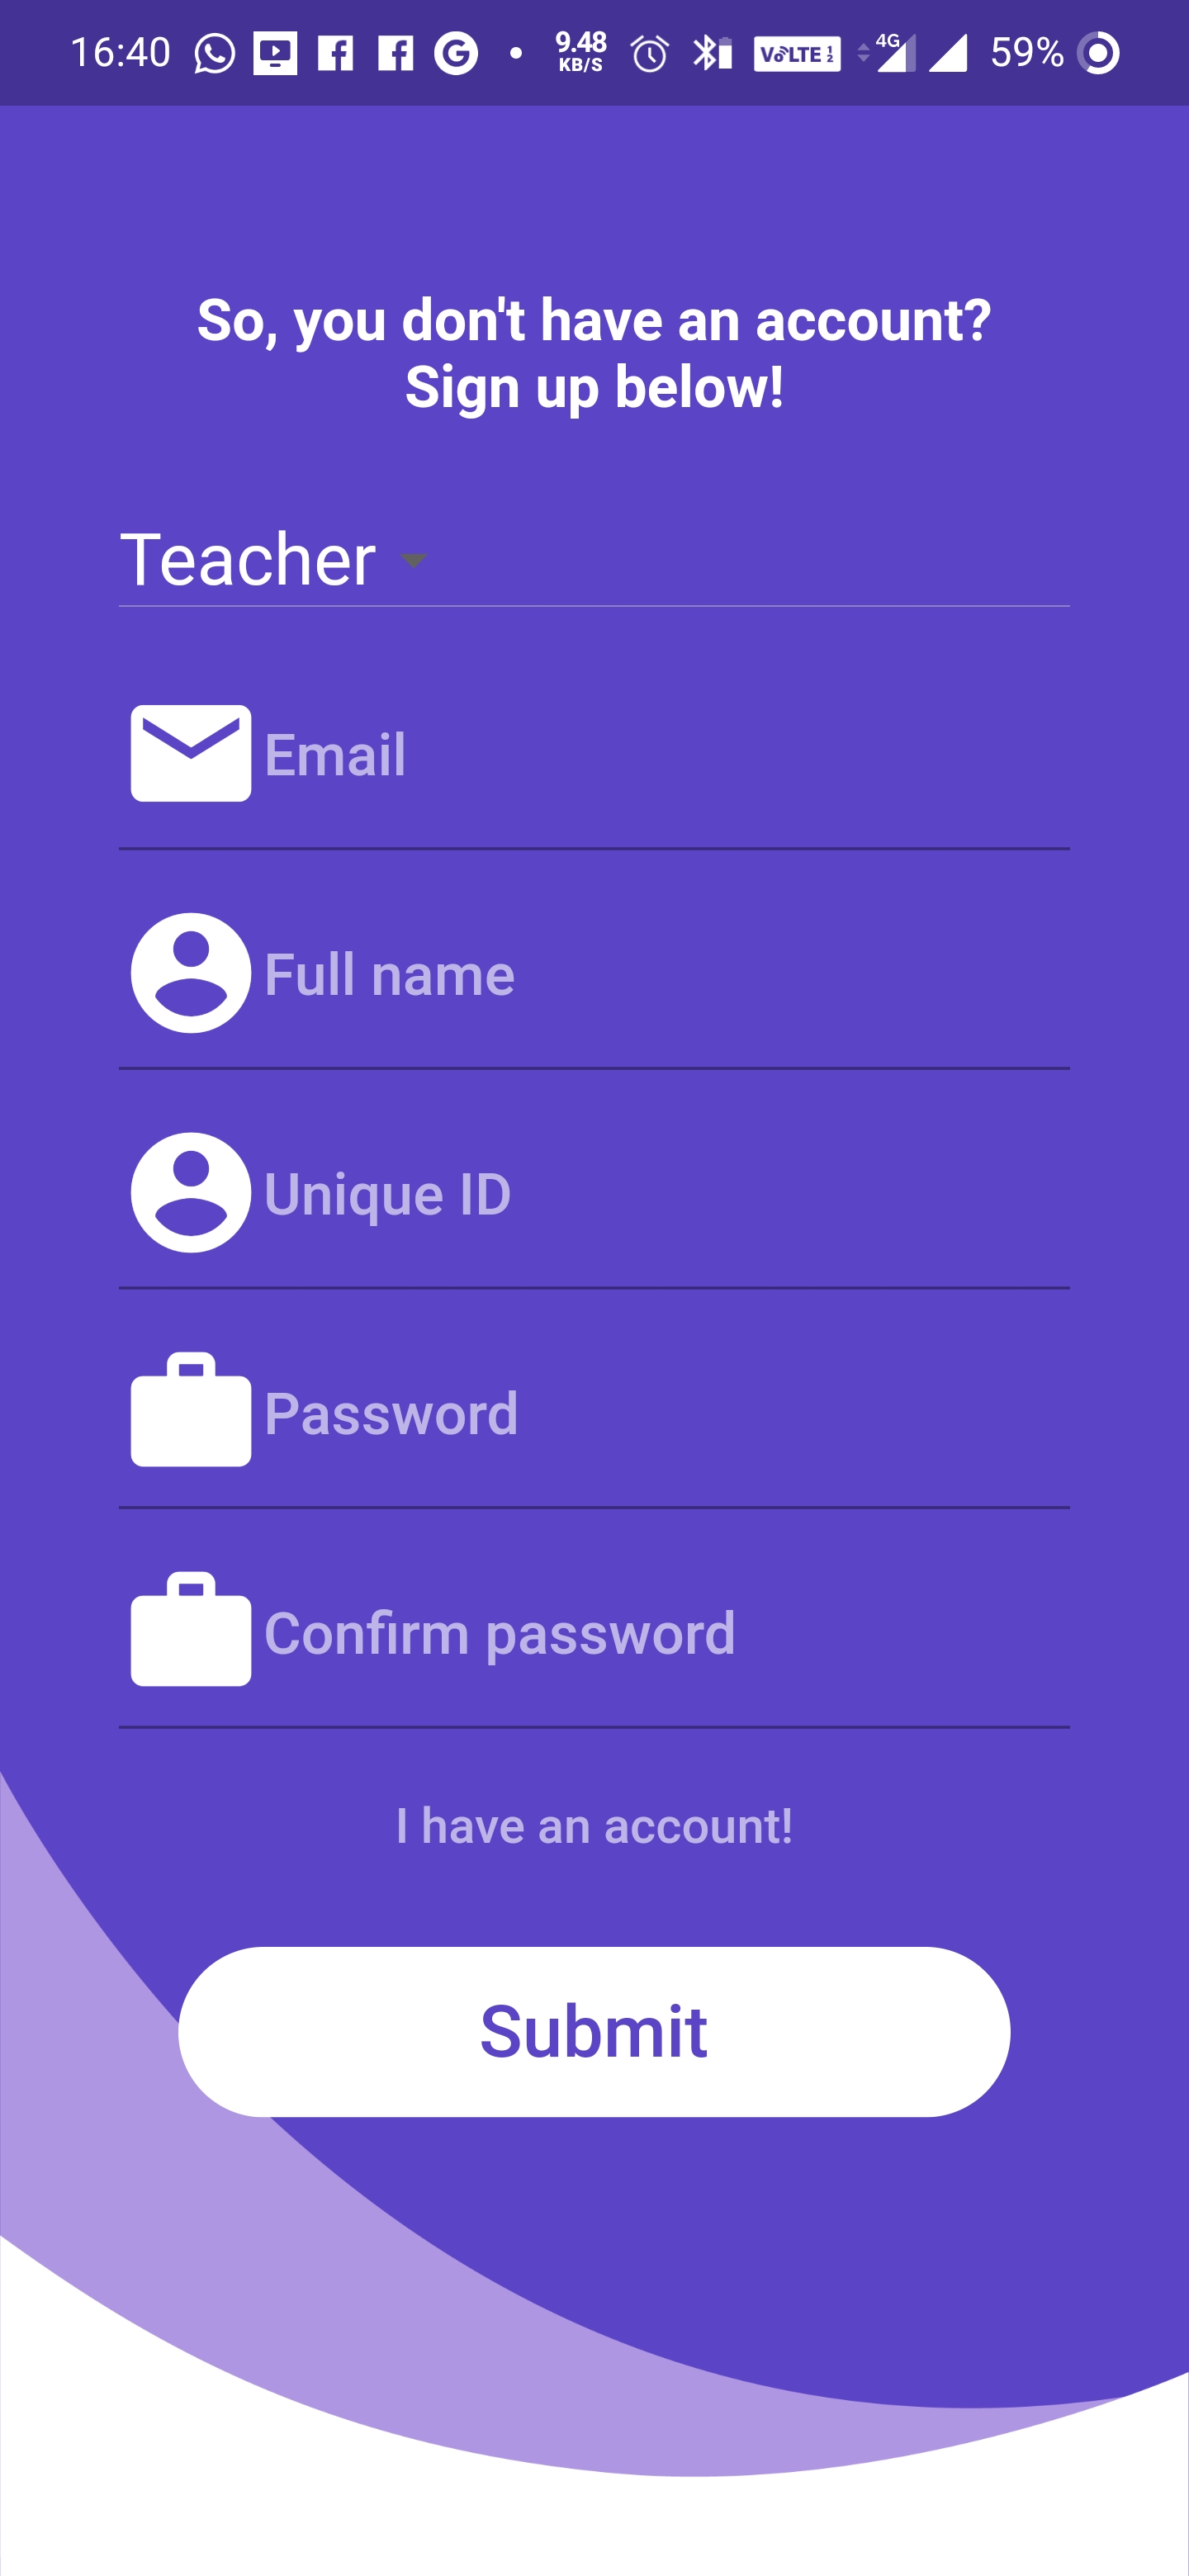
\includegraphics[width=0.40\textwidth]{ProfRegistration.jpg}
    \caption{Student and Professor registration}
    \label{fig:StudentProfReg}
\end{figure}
\begin{figure}[H]
    \centering
    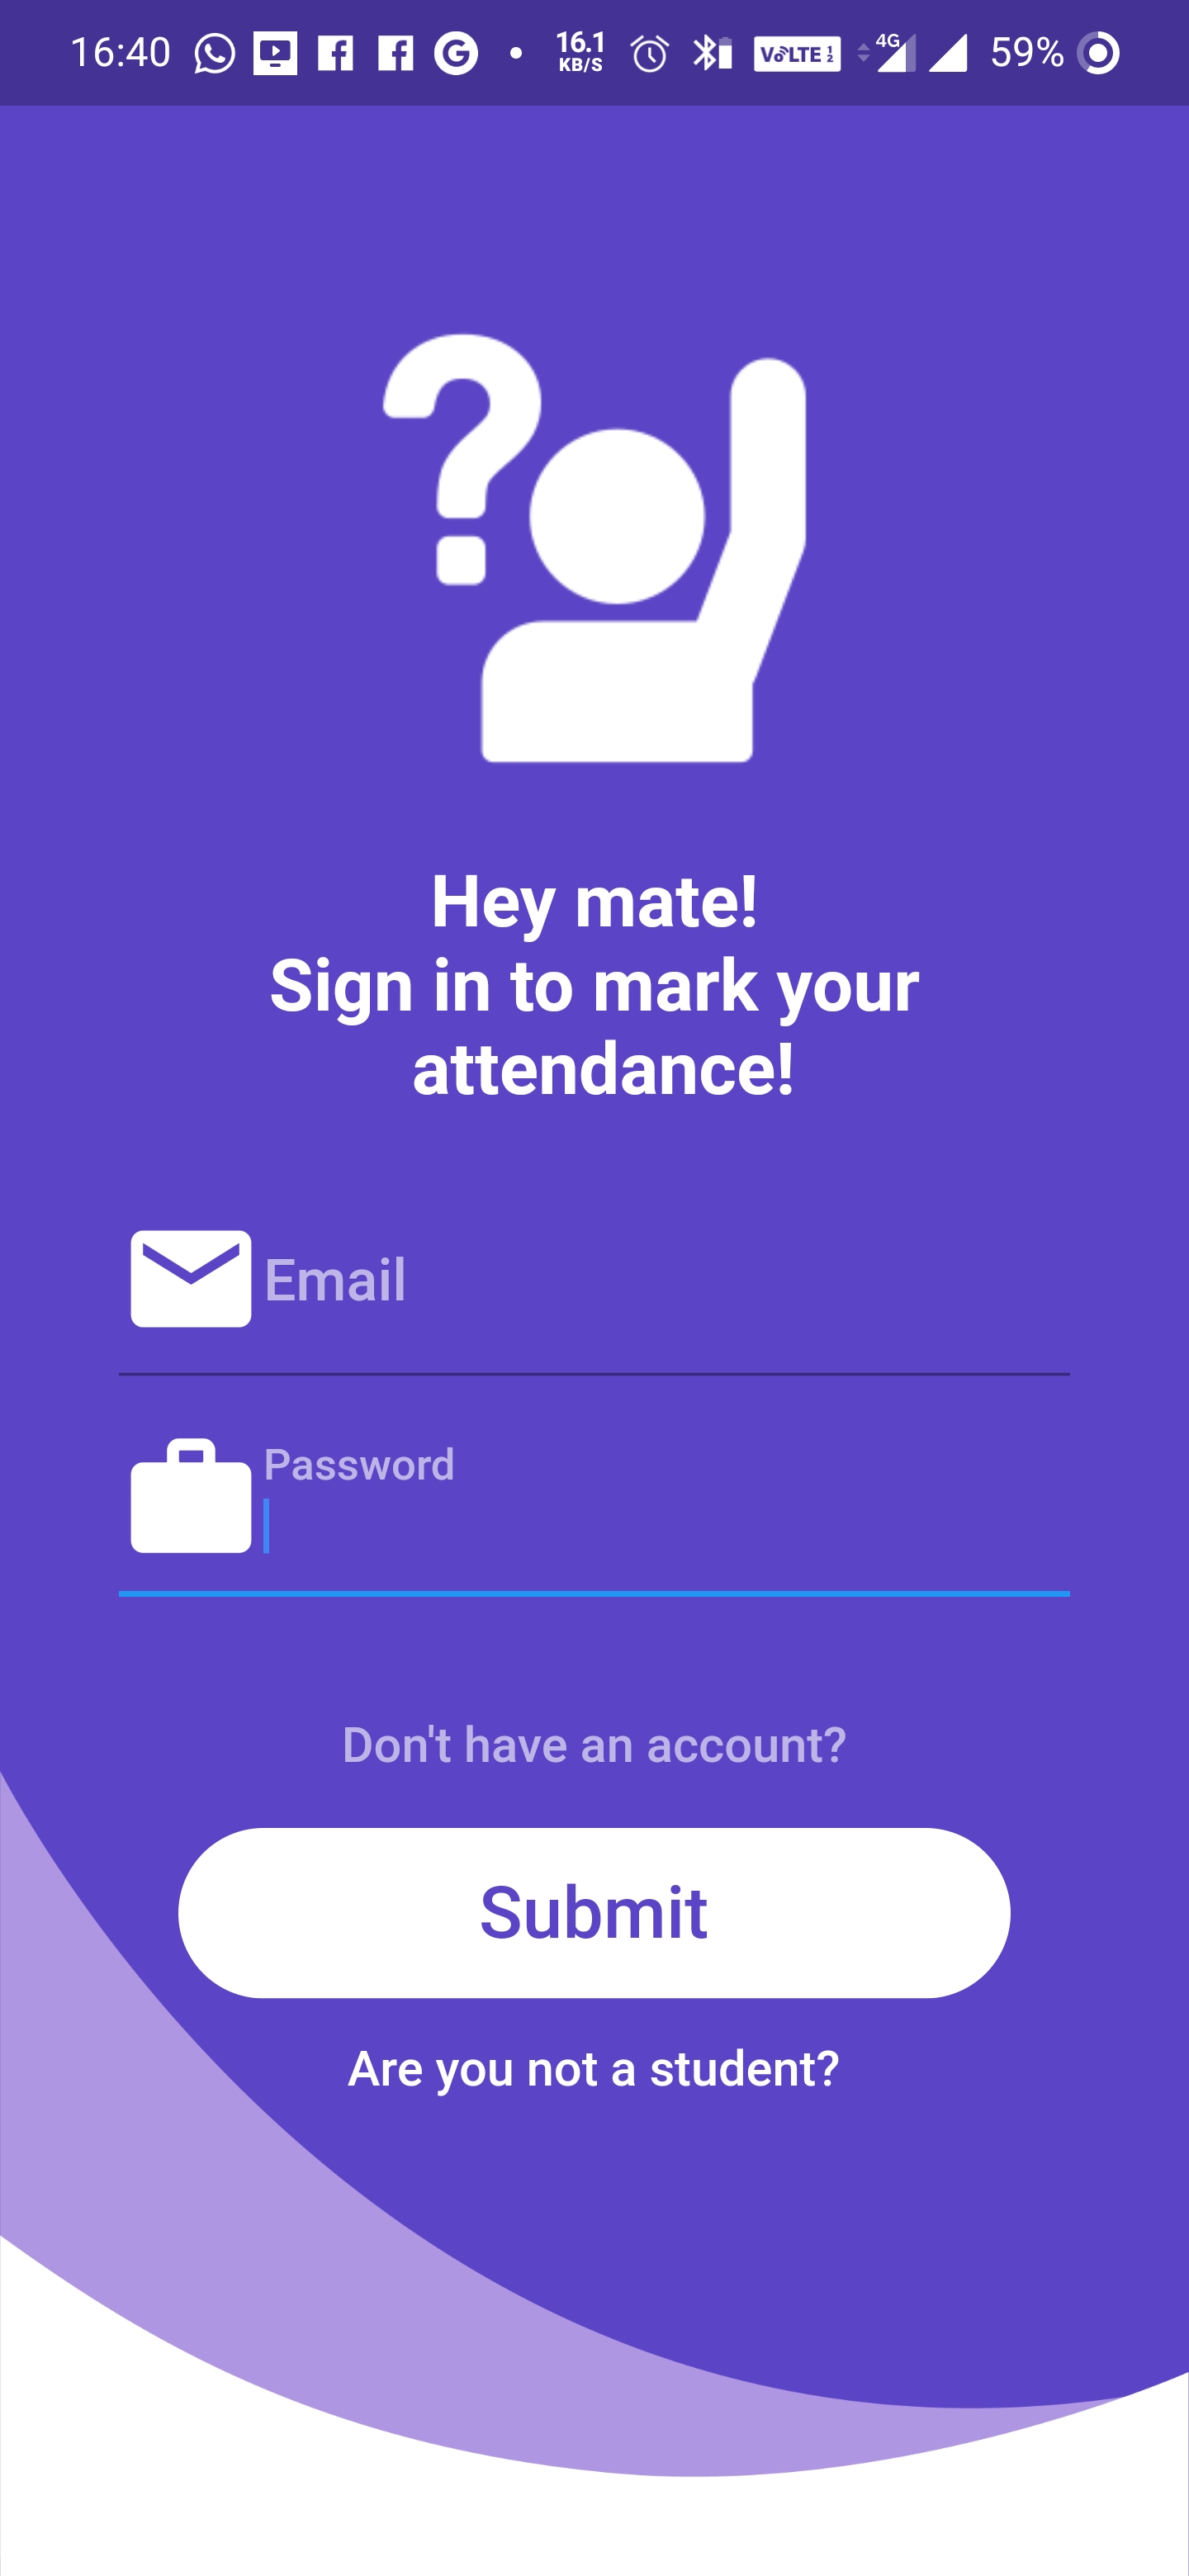
\includegraphics[width=0.40\textwidth]{StudentLogin.jpg}
    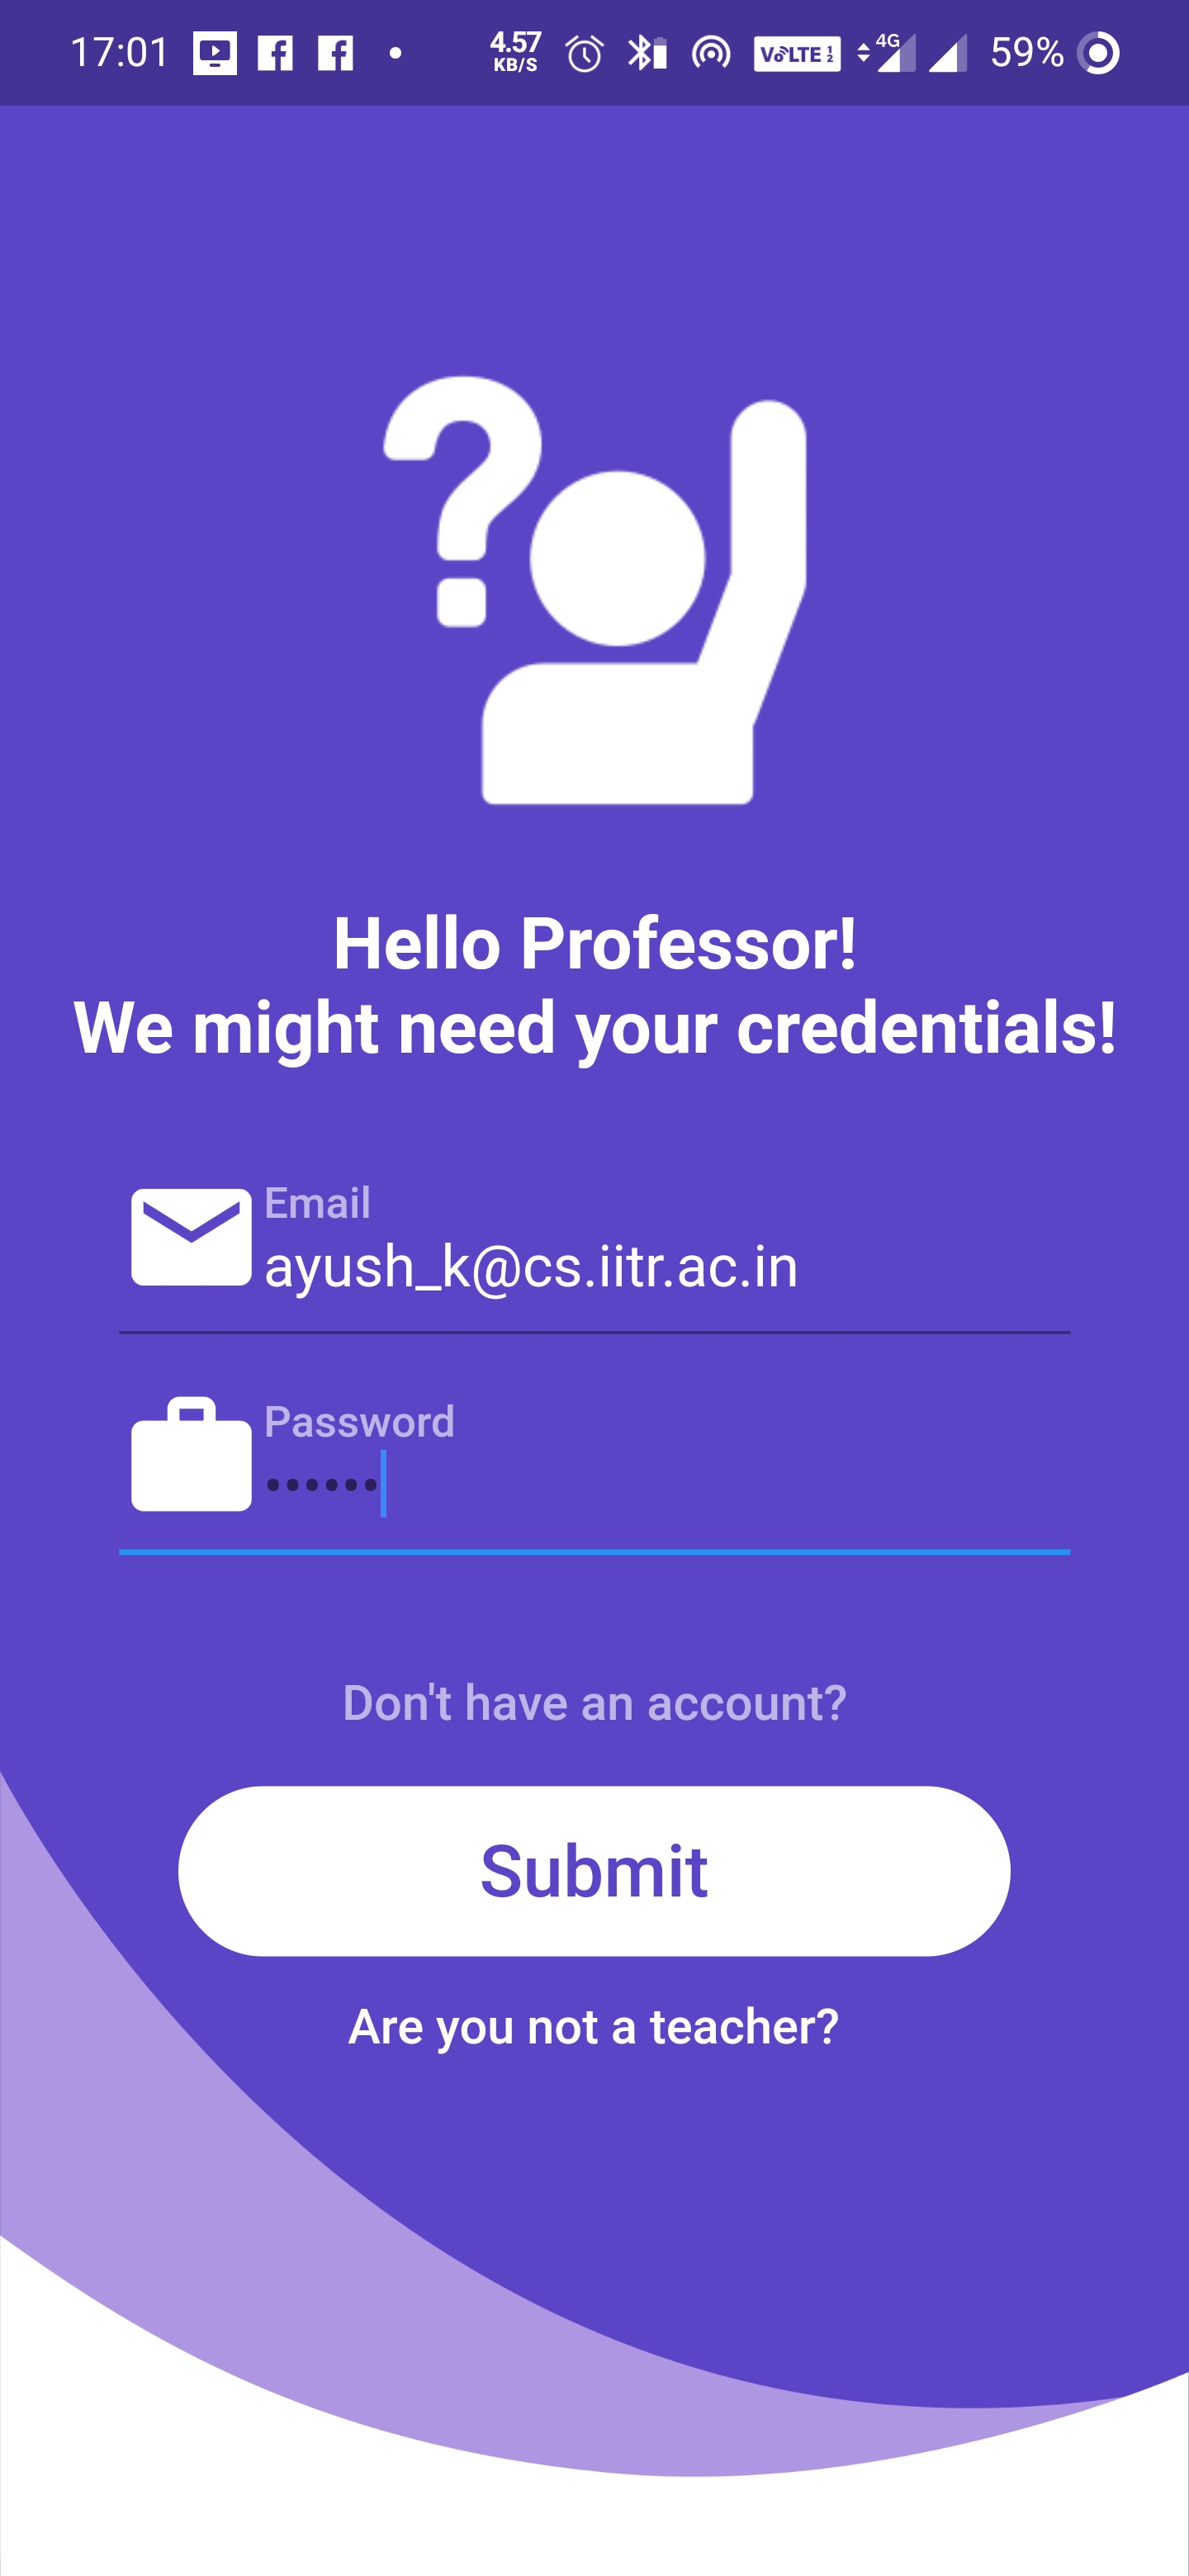
\includegraphics[width=0.40\textwidth]{ProfLogin.jpg}
    \caption{Student and Professor Login}
    \label{fig:StPrLogin}
\end{figure}
\begin{figure}[H]
    \centering
    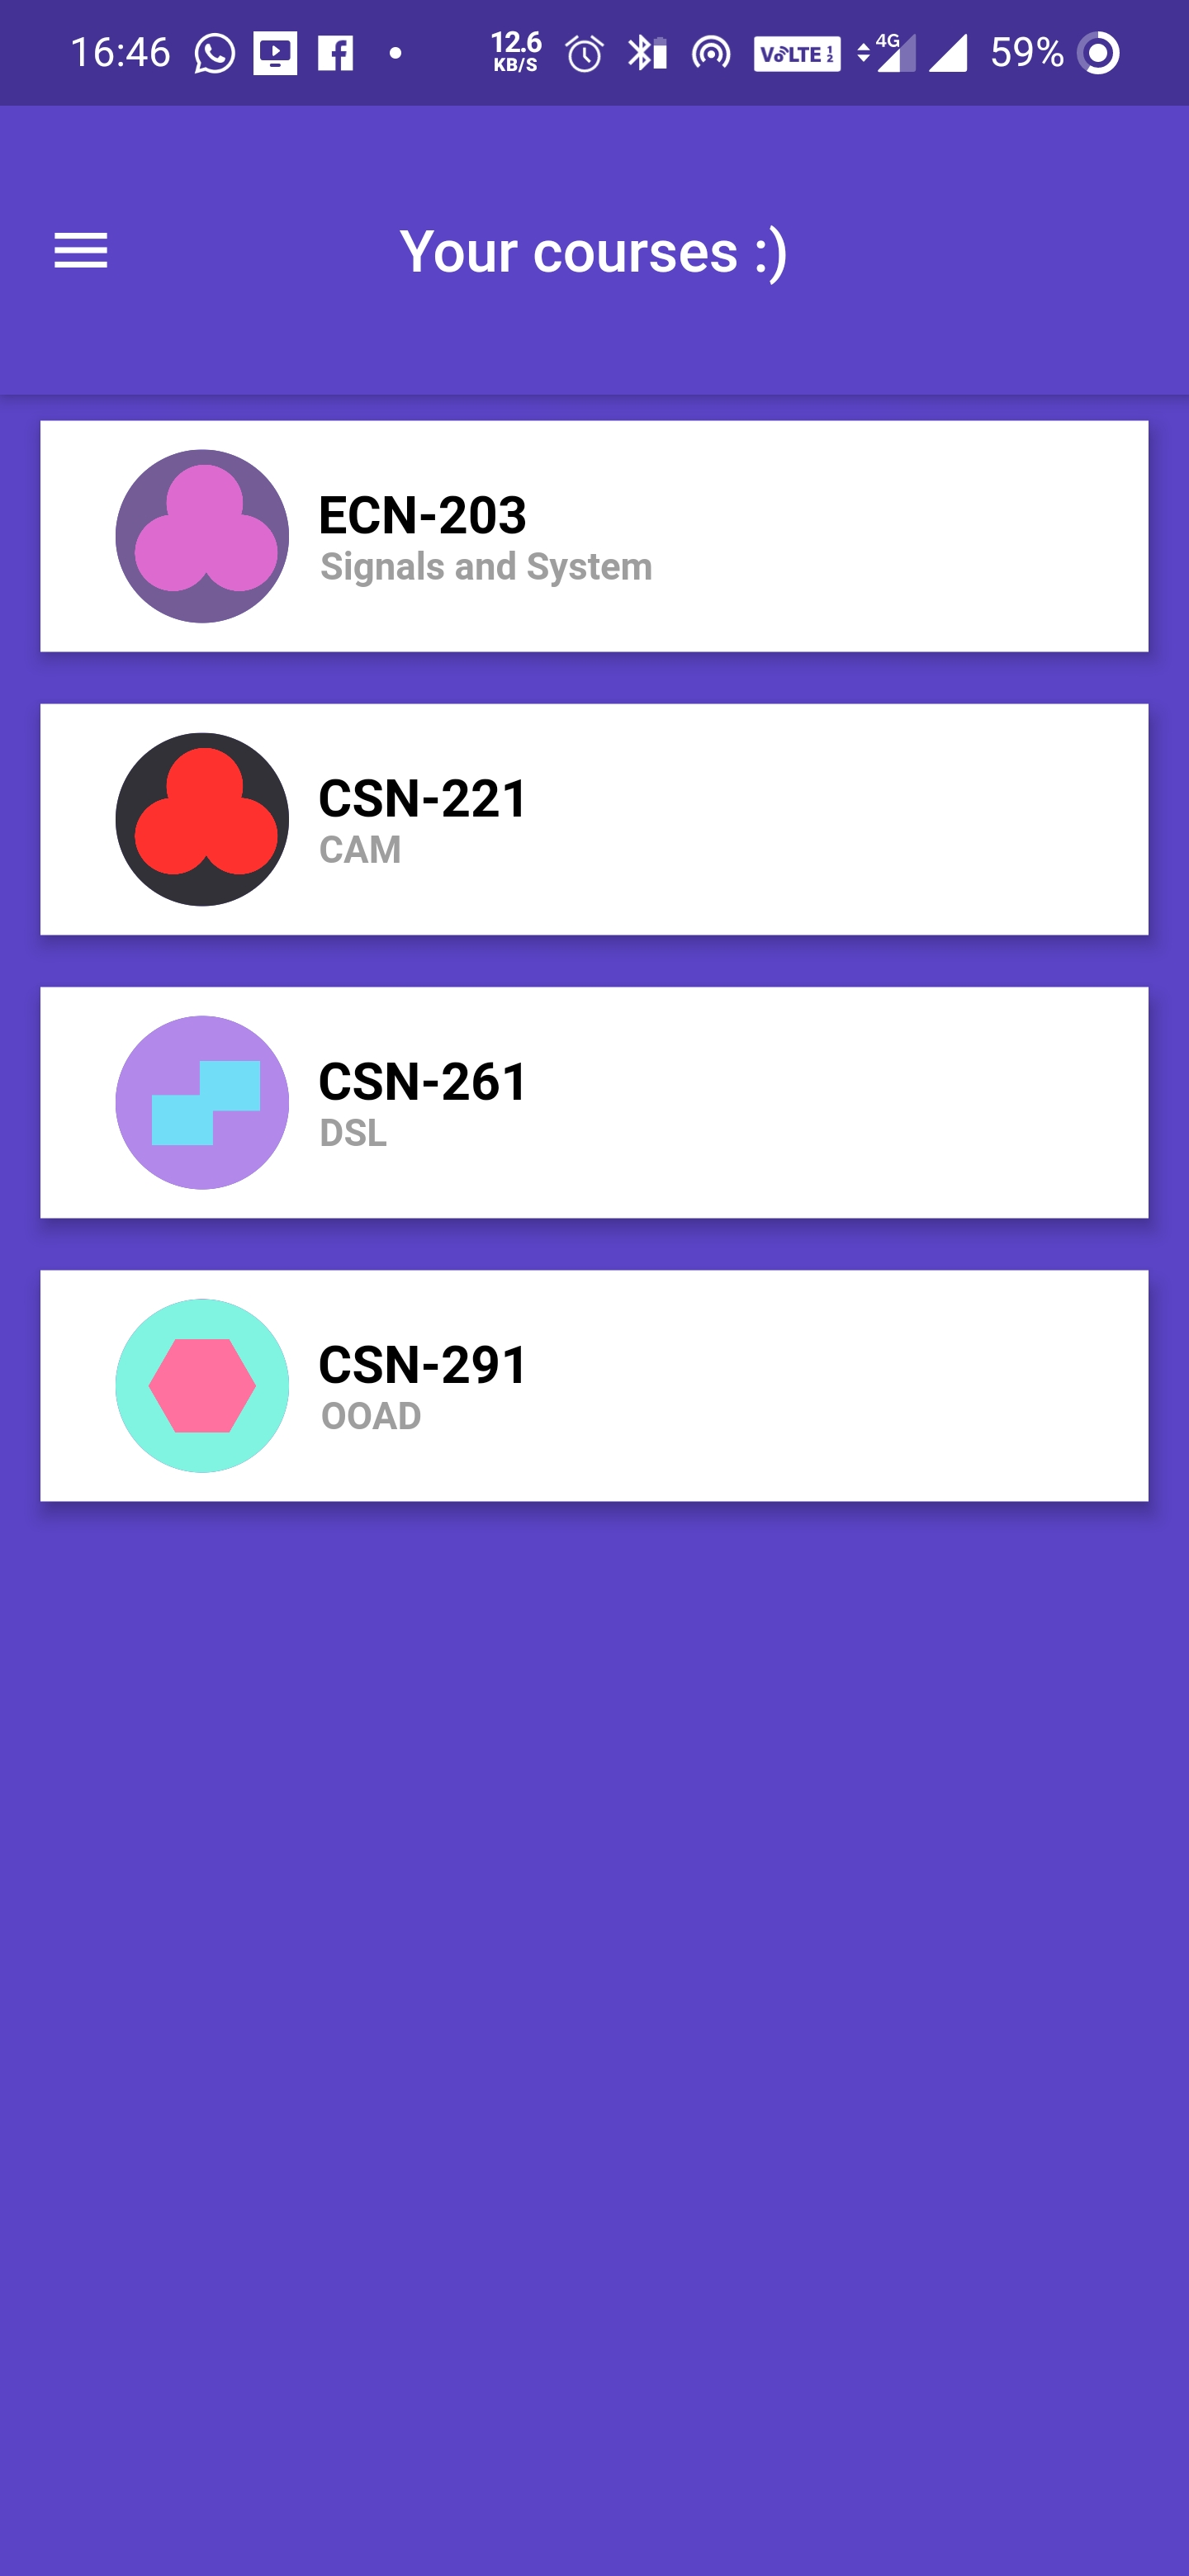
\includegraphics[width=0.40\textwidth]{StudentsCourses.jpg}
    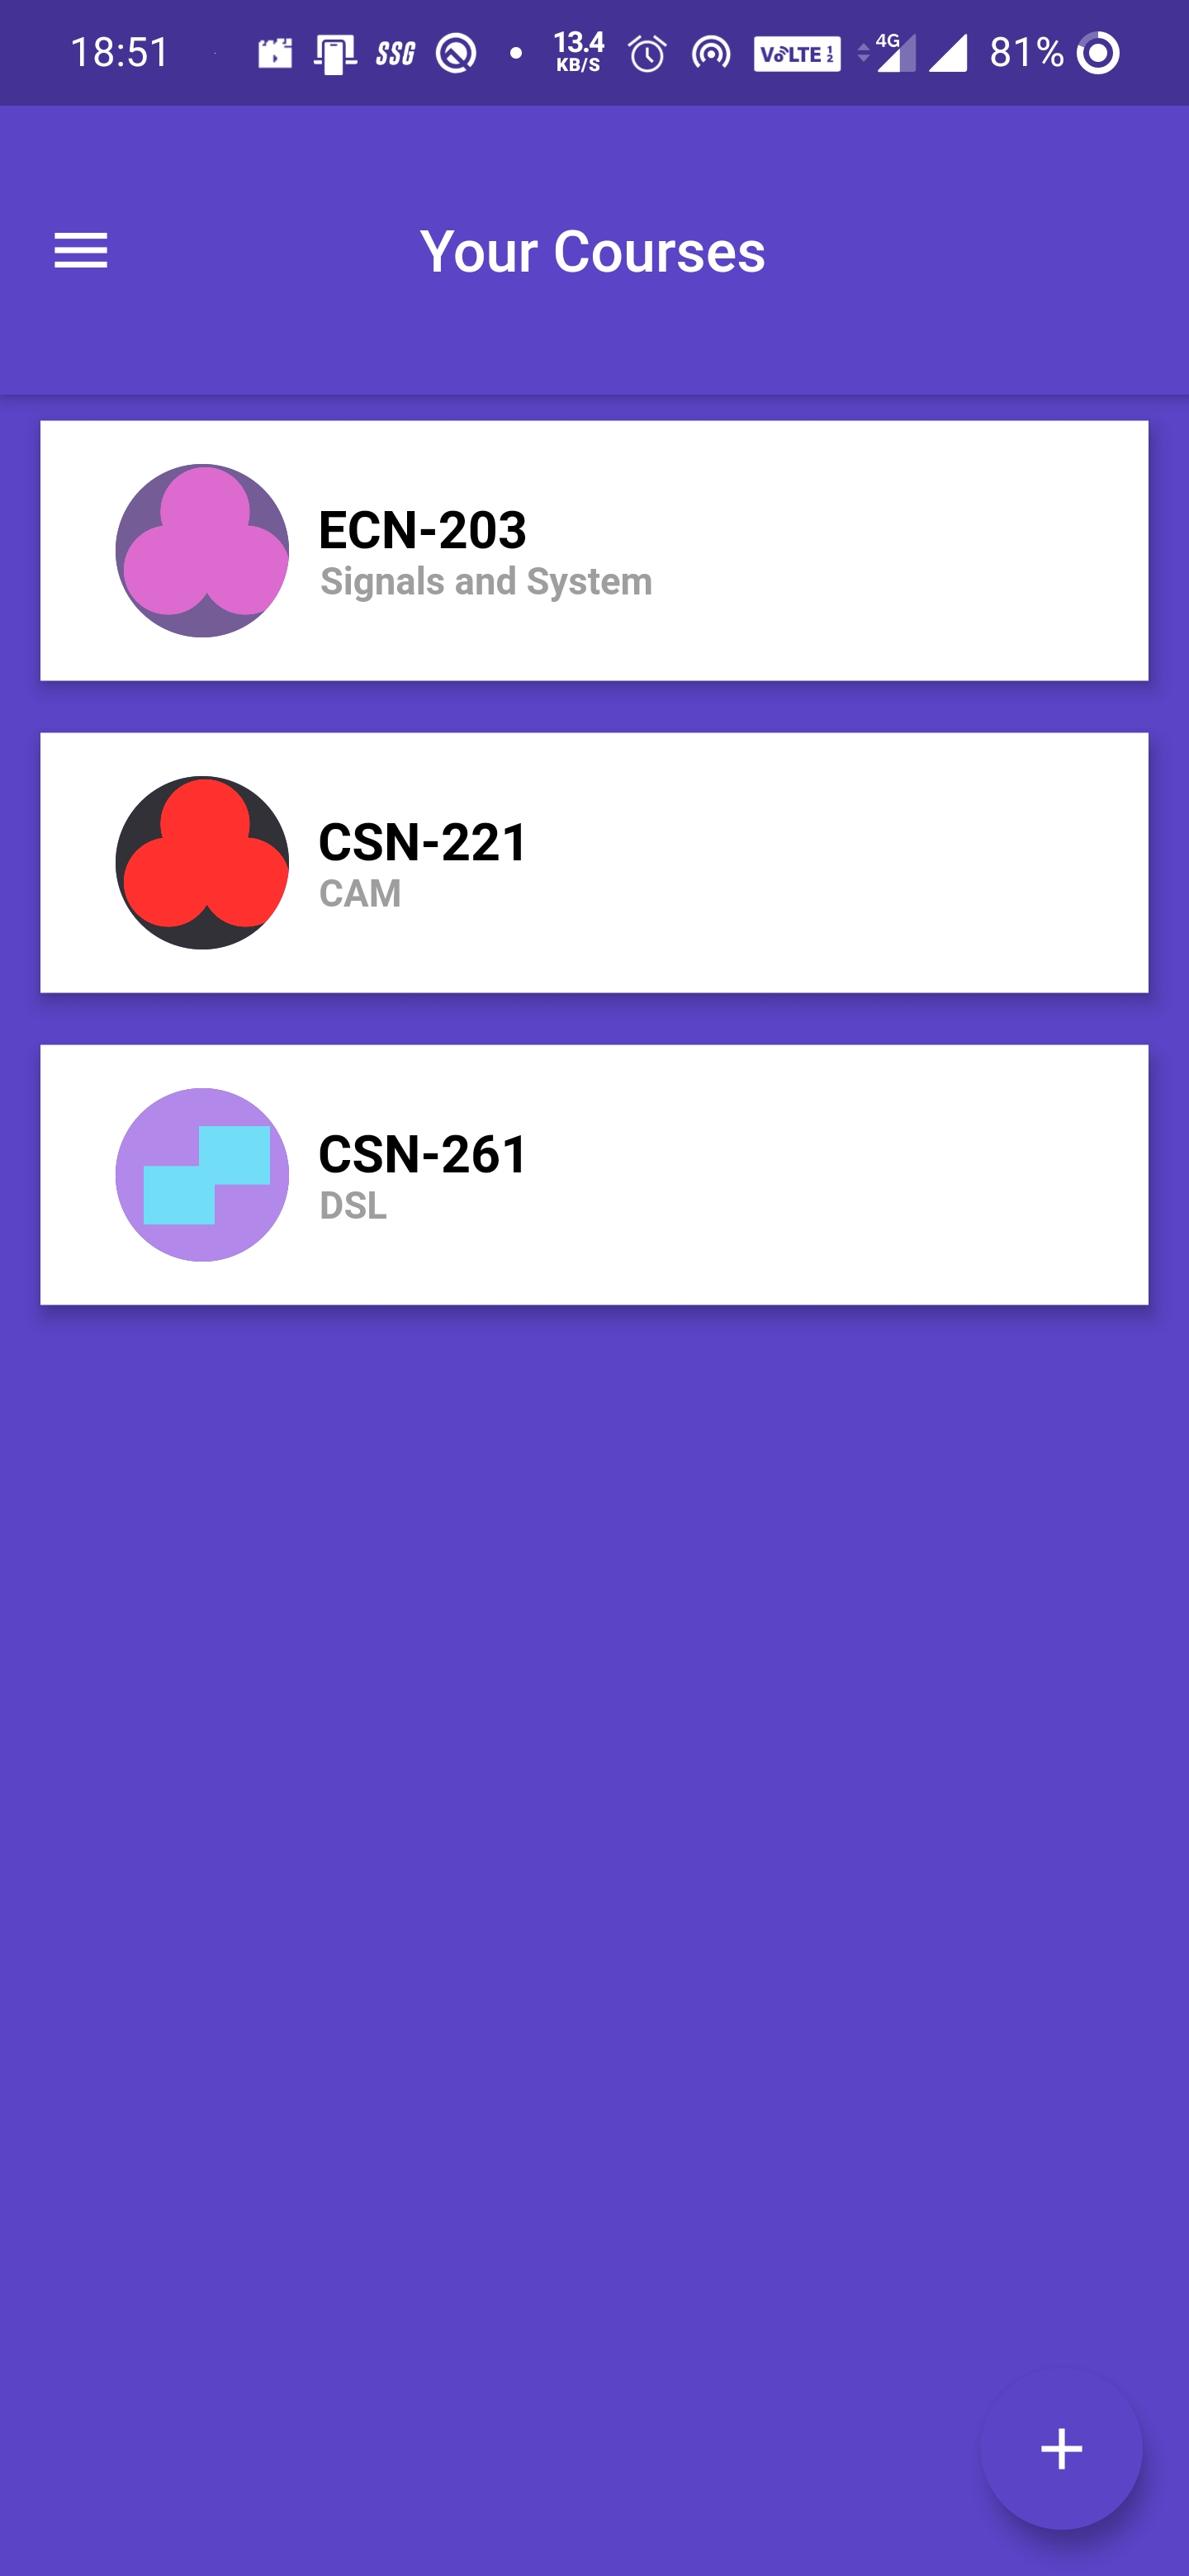
\includegraphics[width=0.40\textwidth]{ProfCourses.jpg}
    \caption{Student and Professor Home Page}
    \label{fig:StPrCourses}
\end{figure}
\begin{figure}[H]
    \centering
    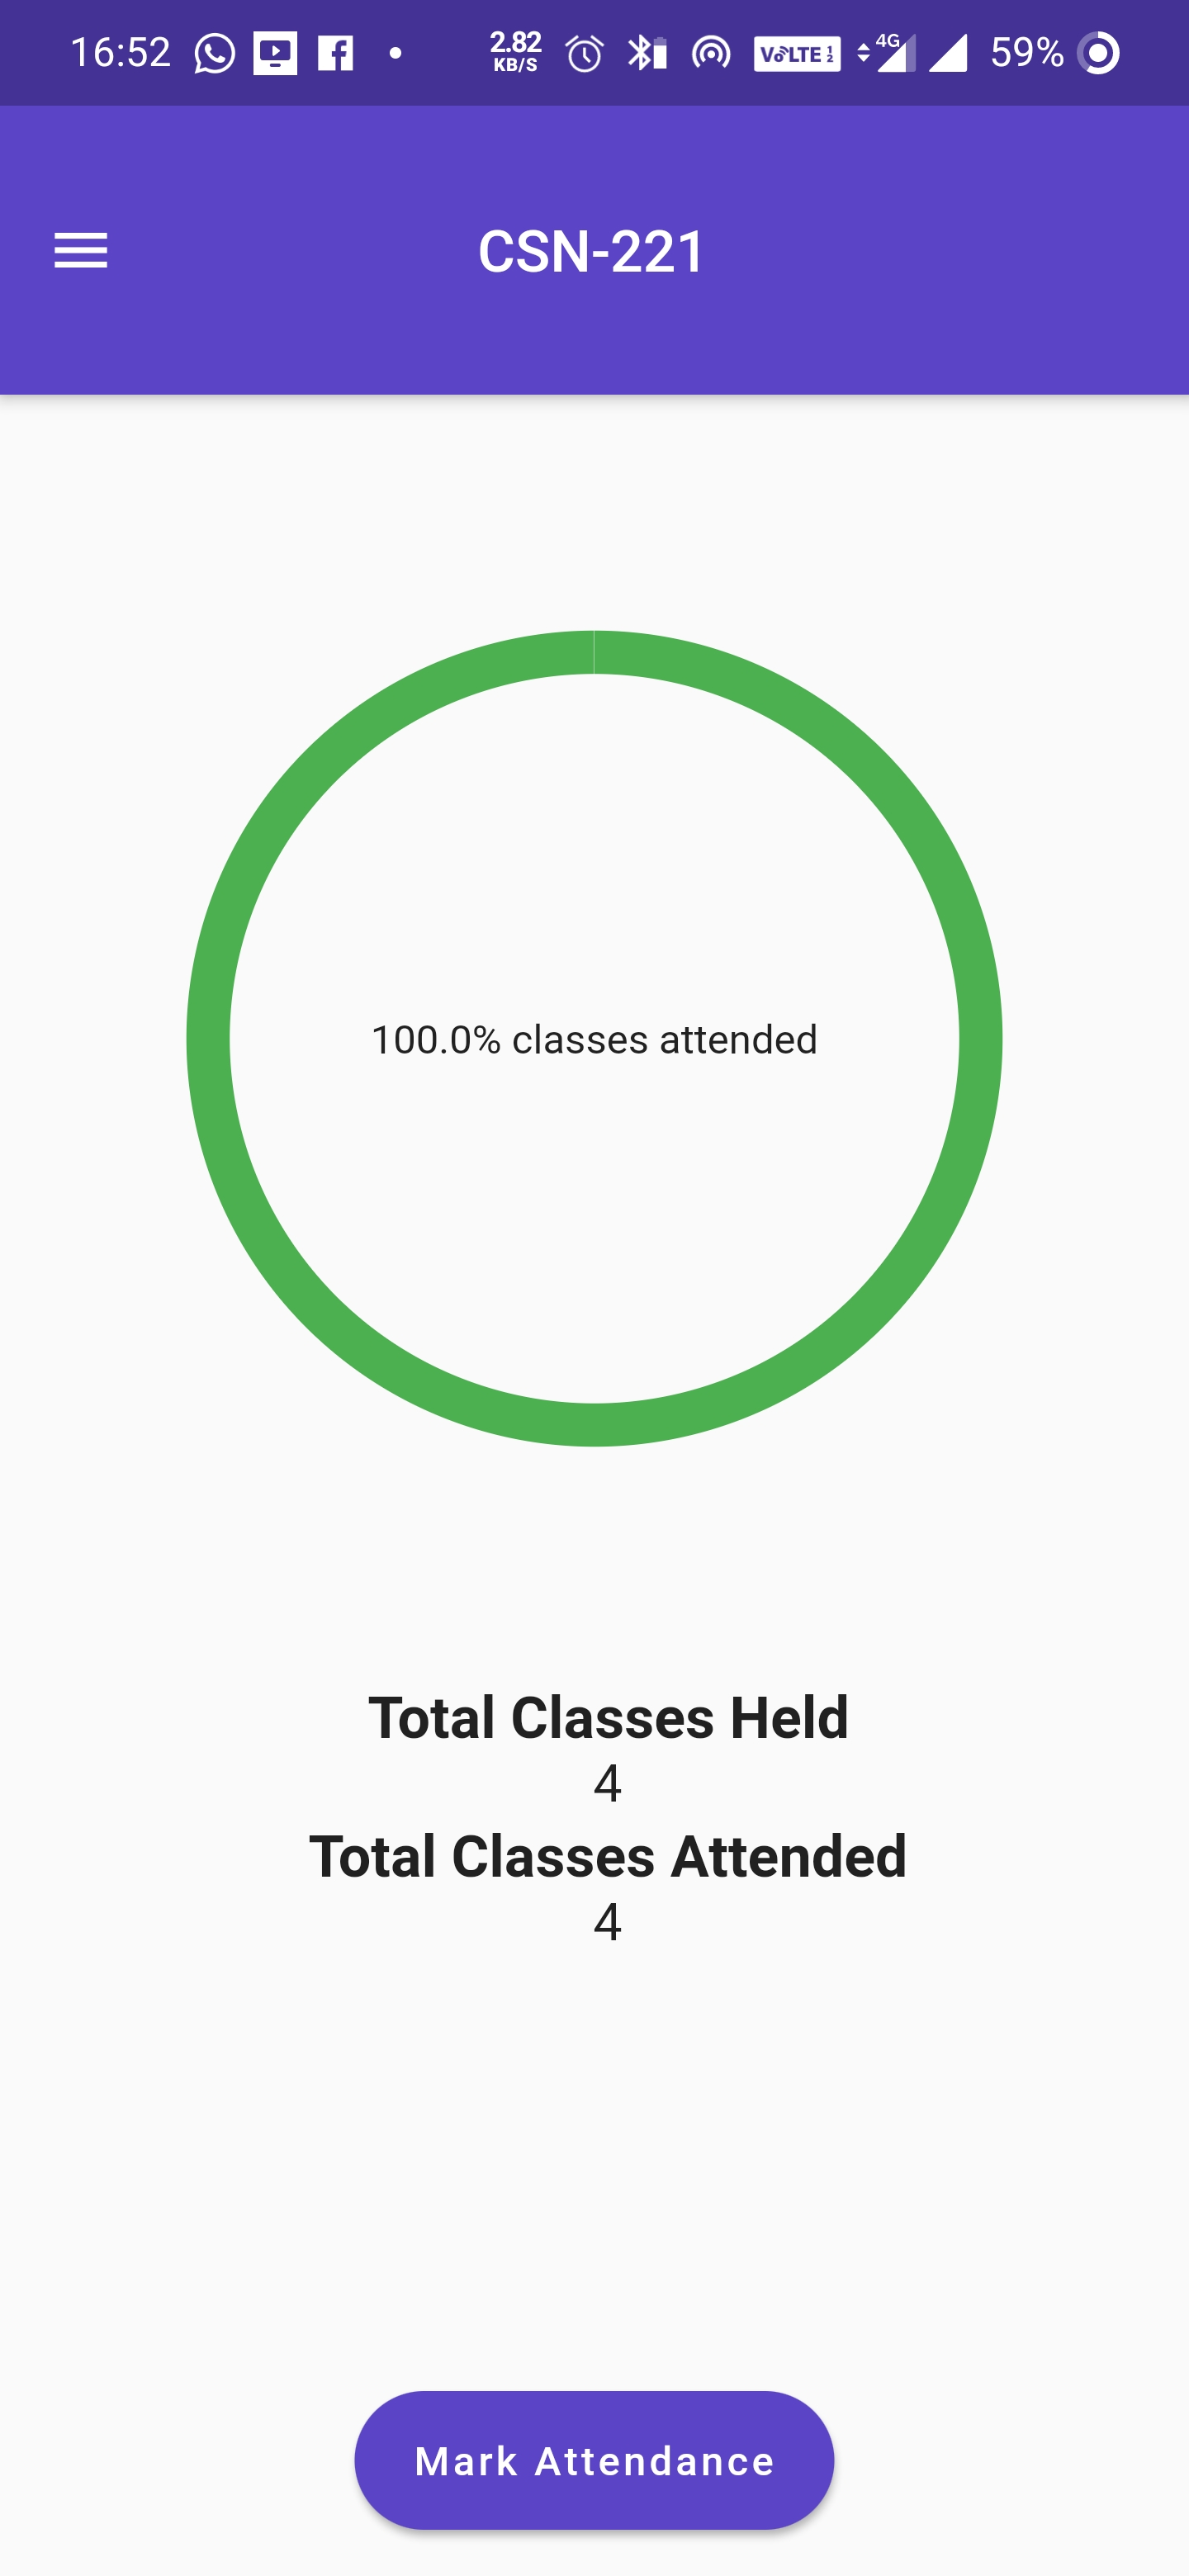
\includegraphics[width=0.40\textwidth]{AttGreenbar.jpg}
    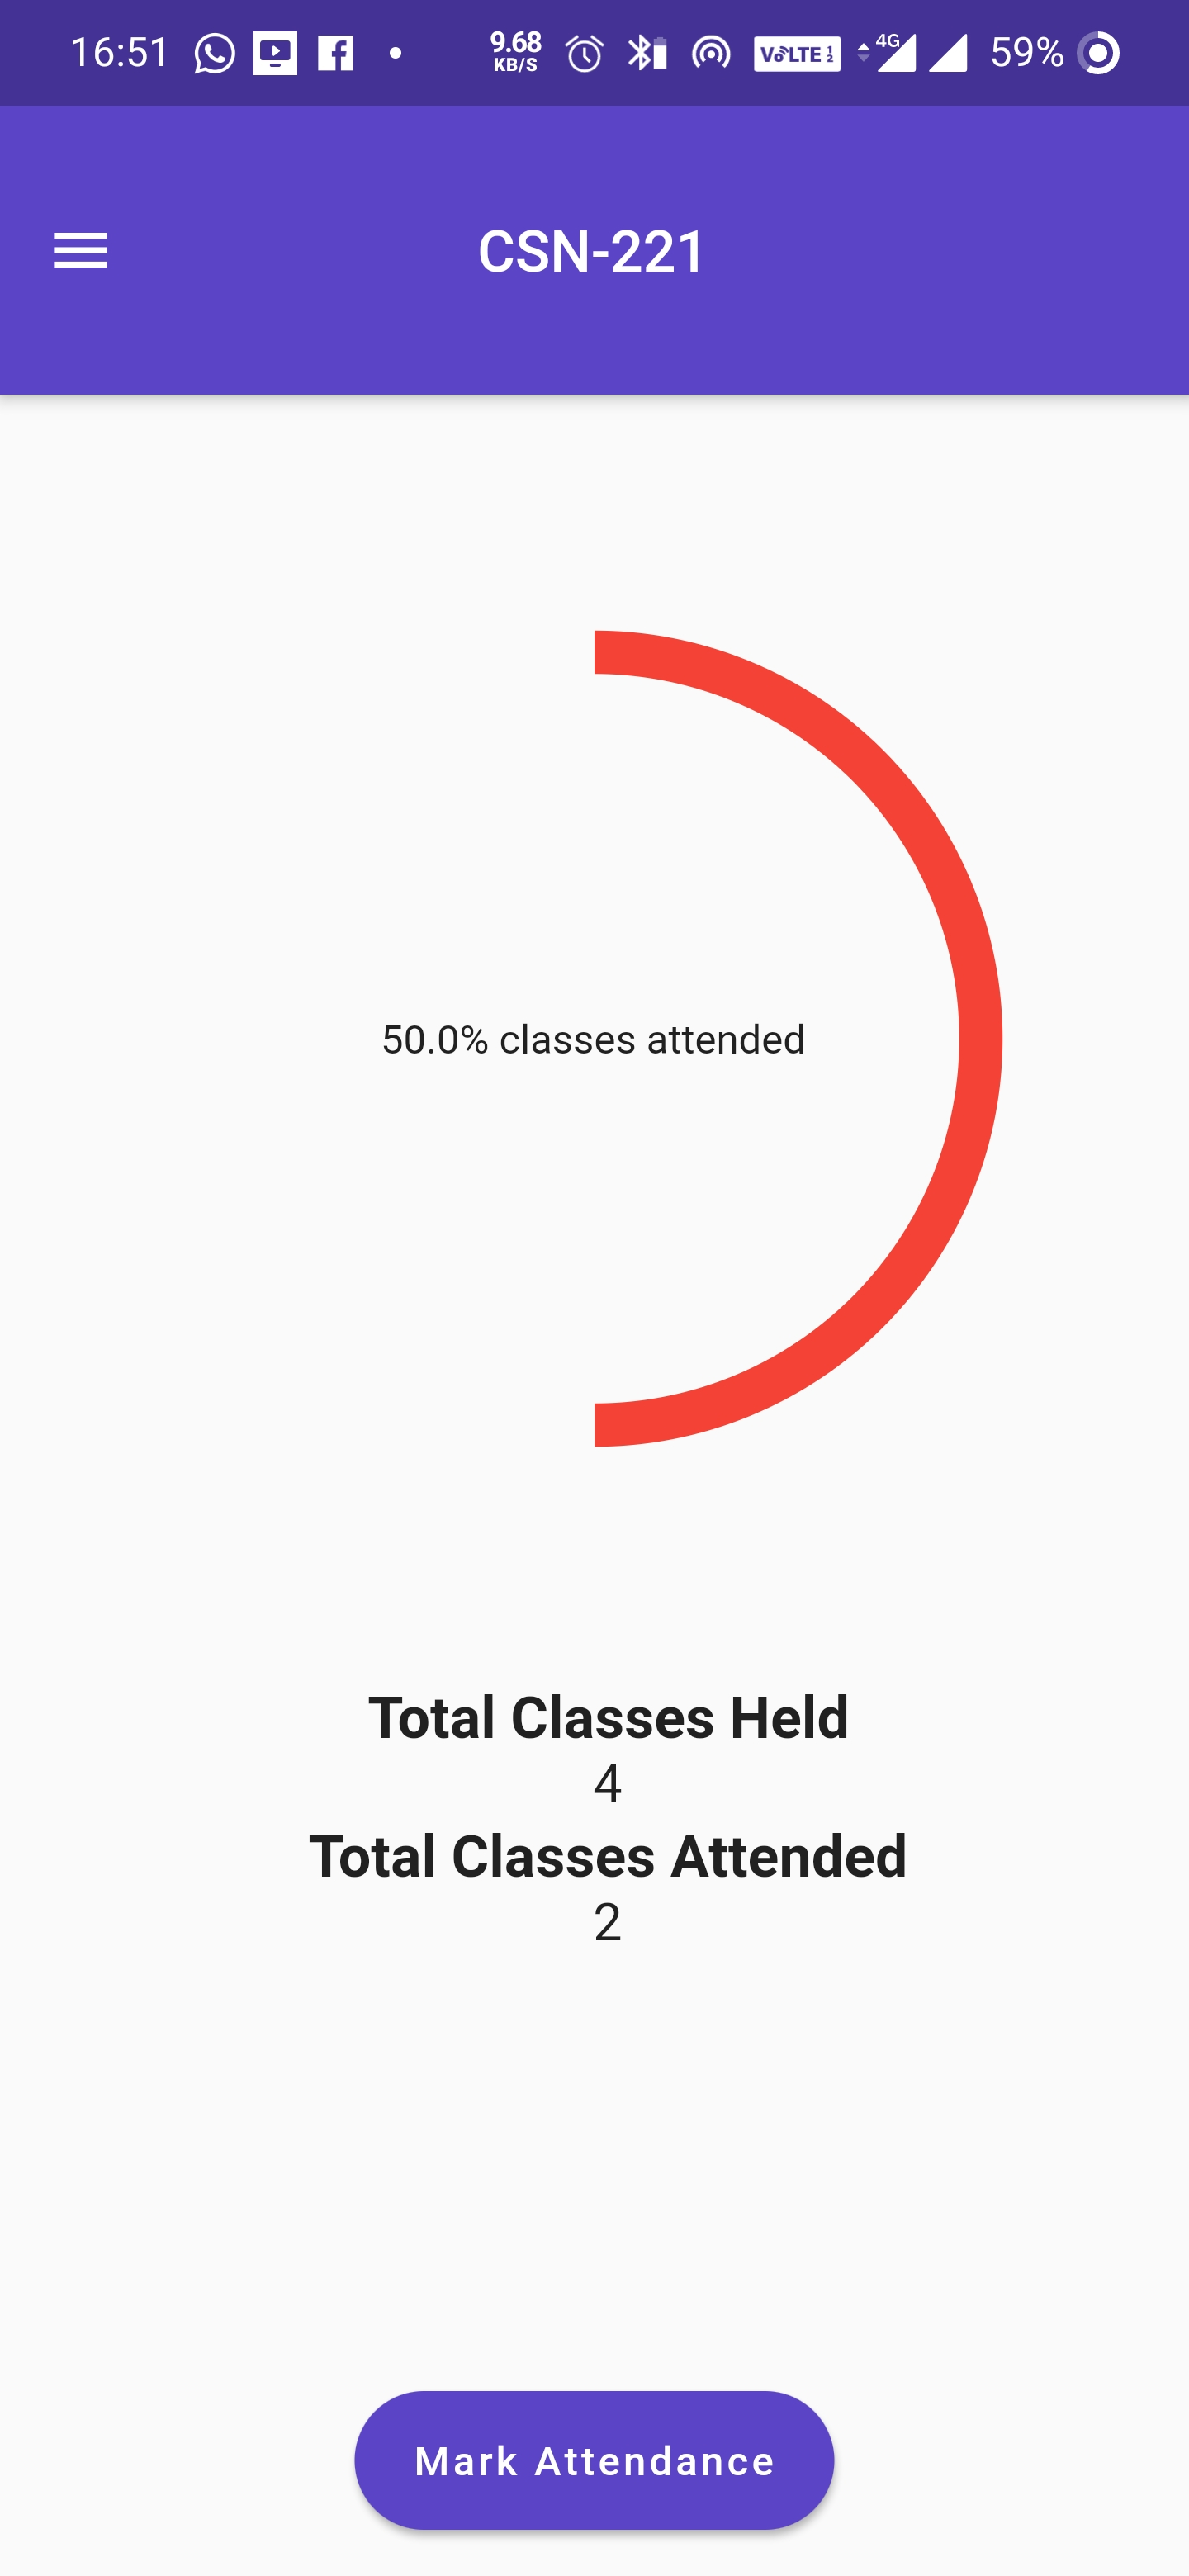
\includegraphics[width=0.40\textwidth]{AttRedbar.jpg}
    \caption{Attendance bar}
    \label{fig:Attbar}
\end{figure}
\begin{figure}[H]
    \centering
    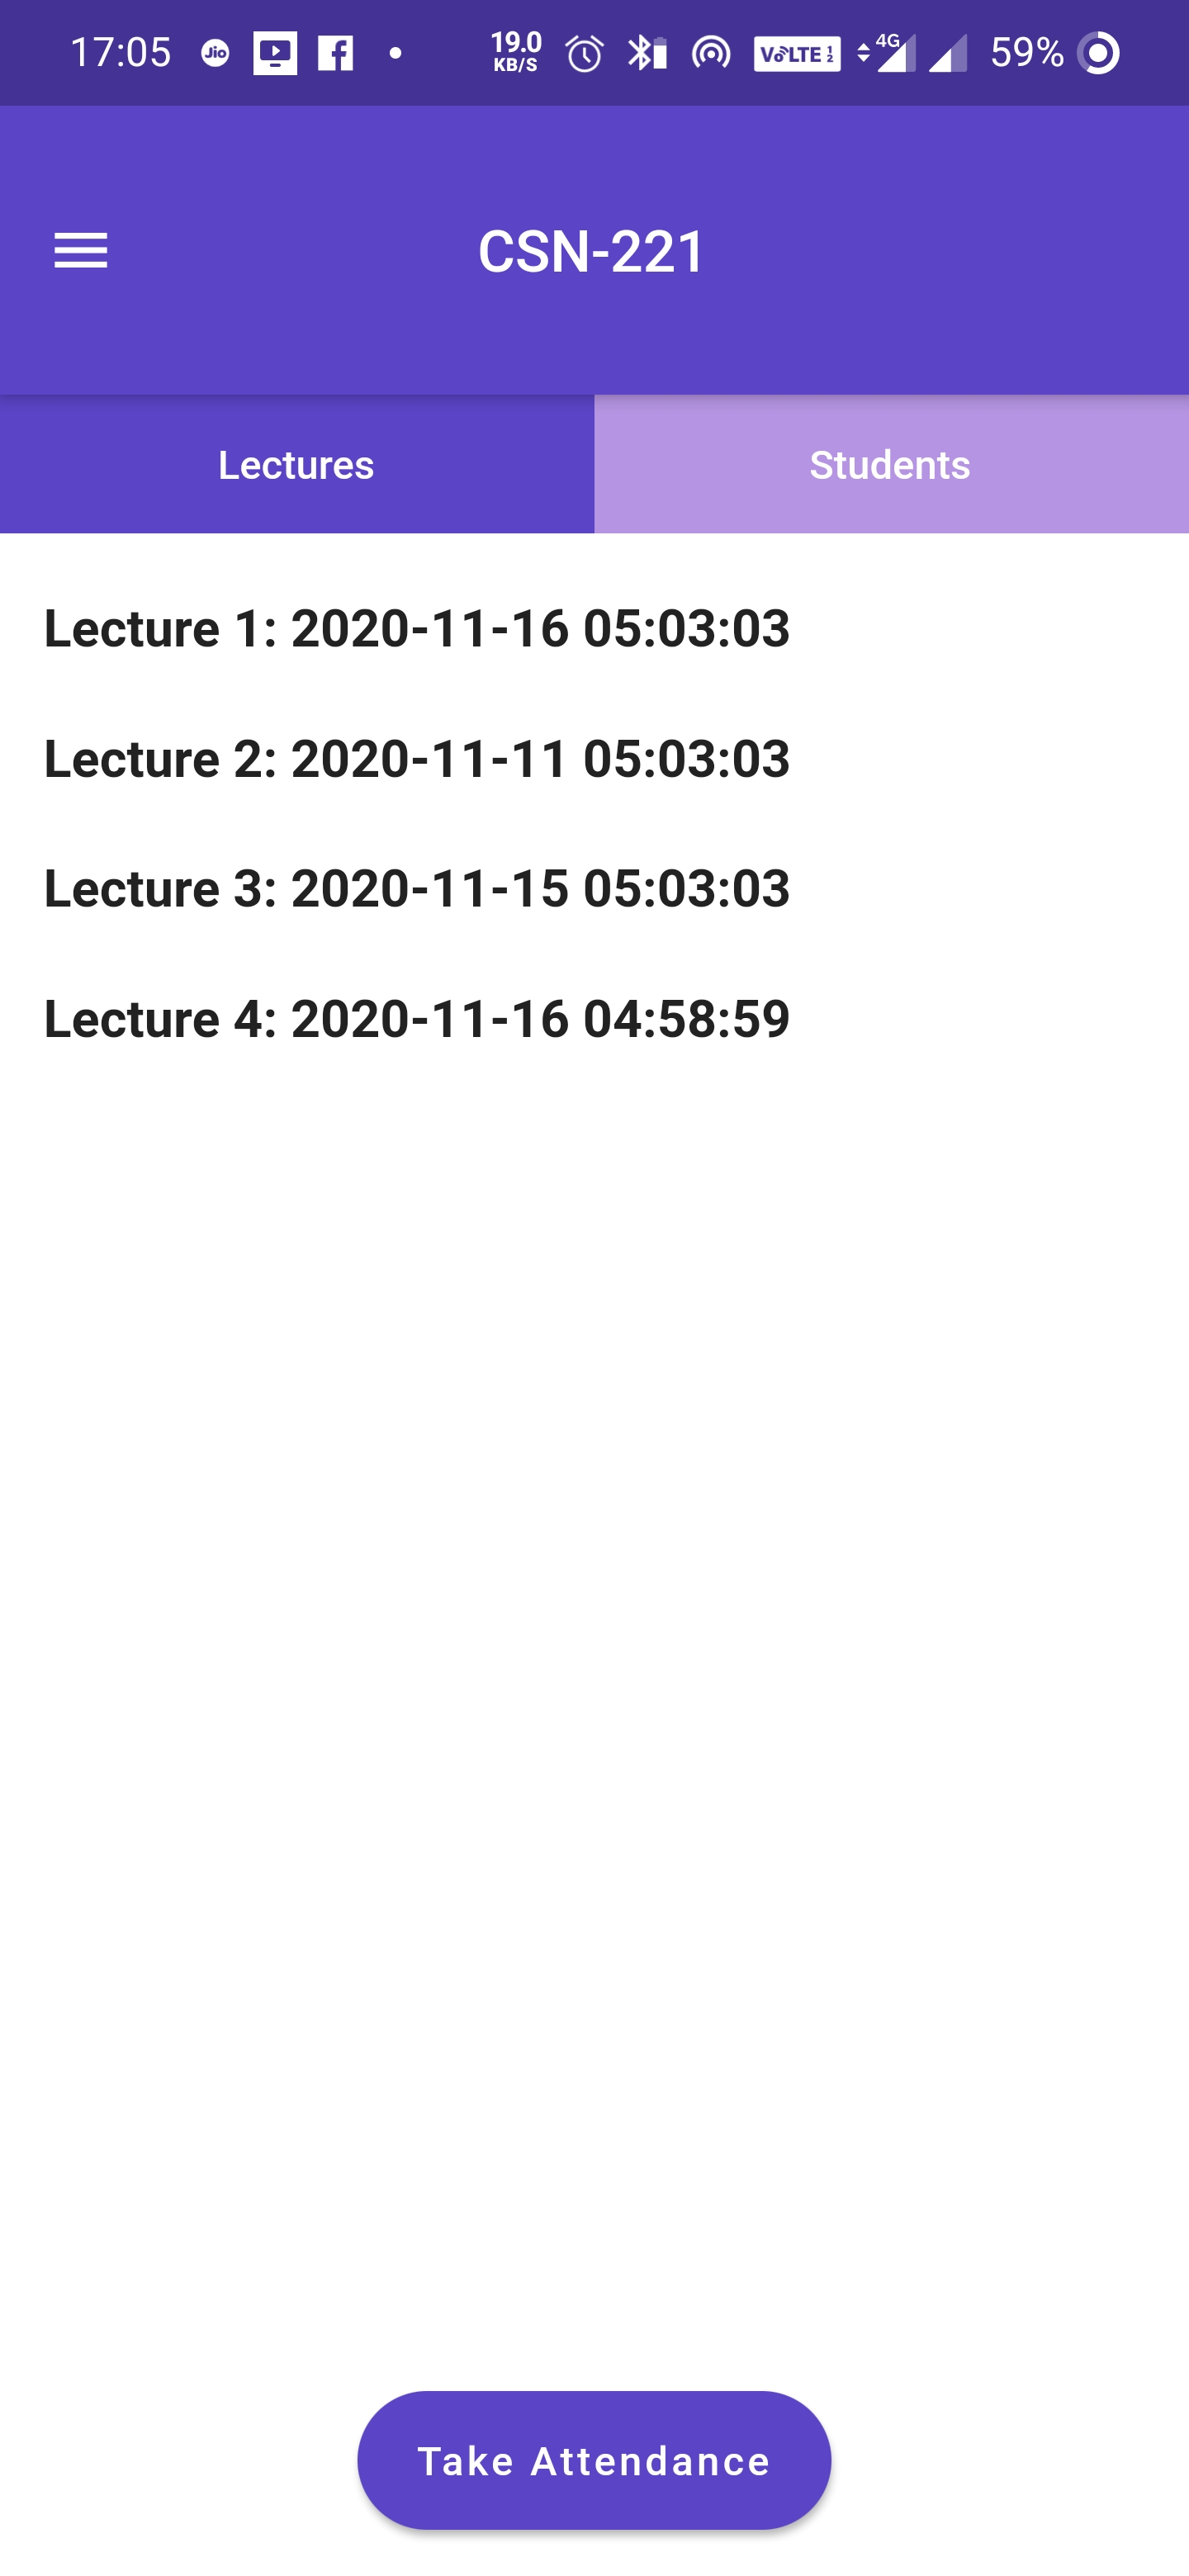
\includegraphics[width=0.40\textwidth]{Students.jpg}
    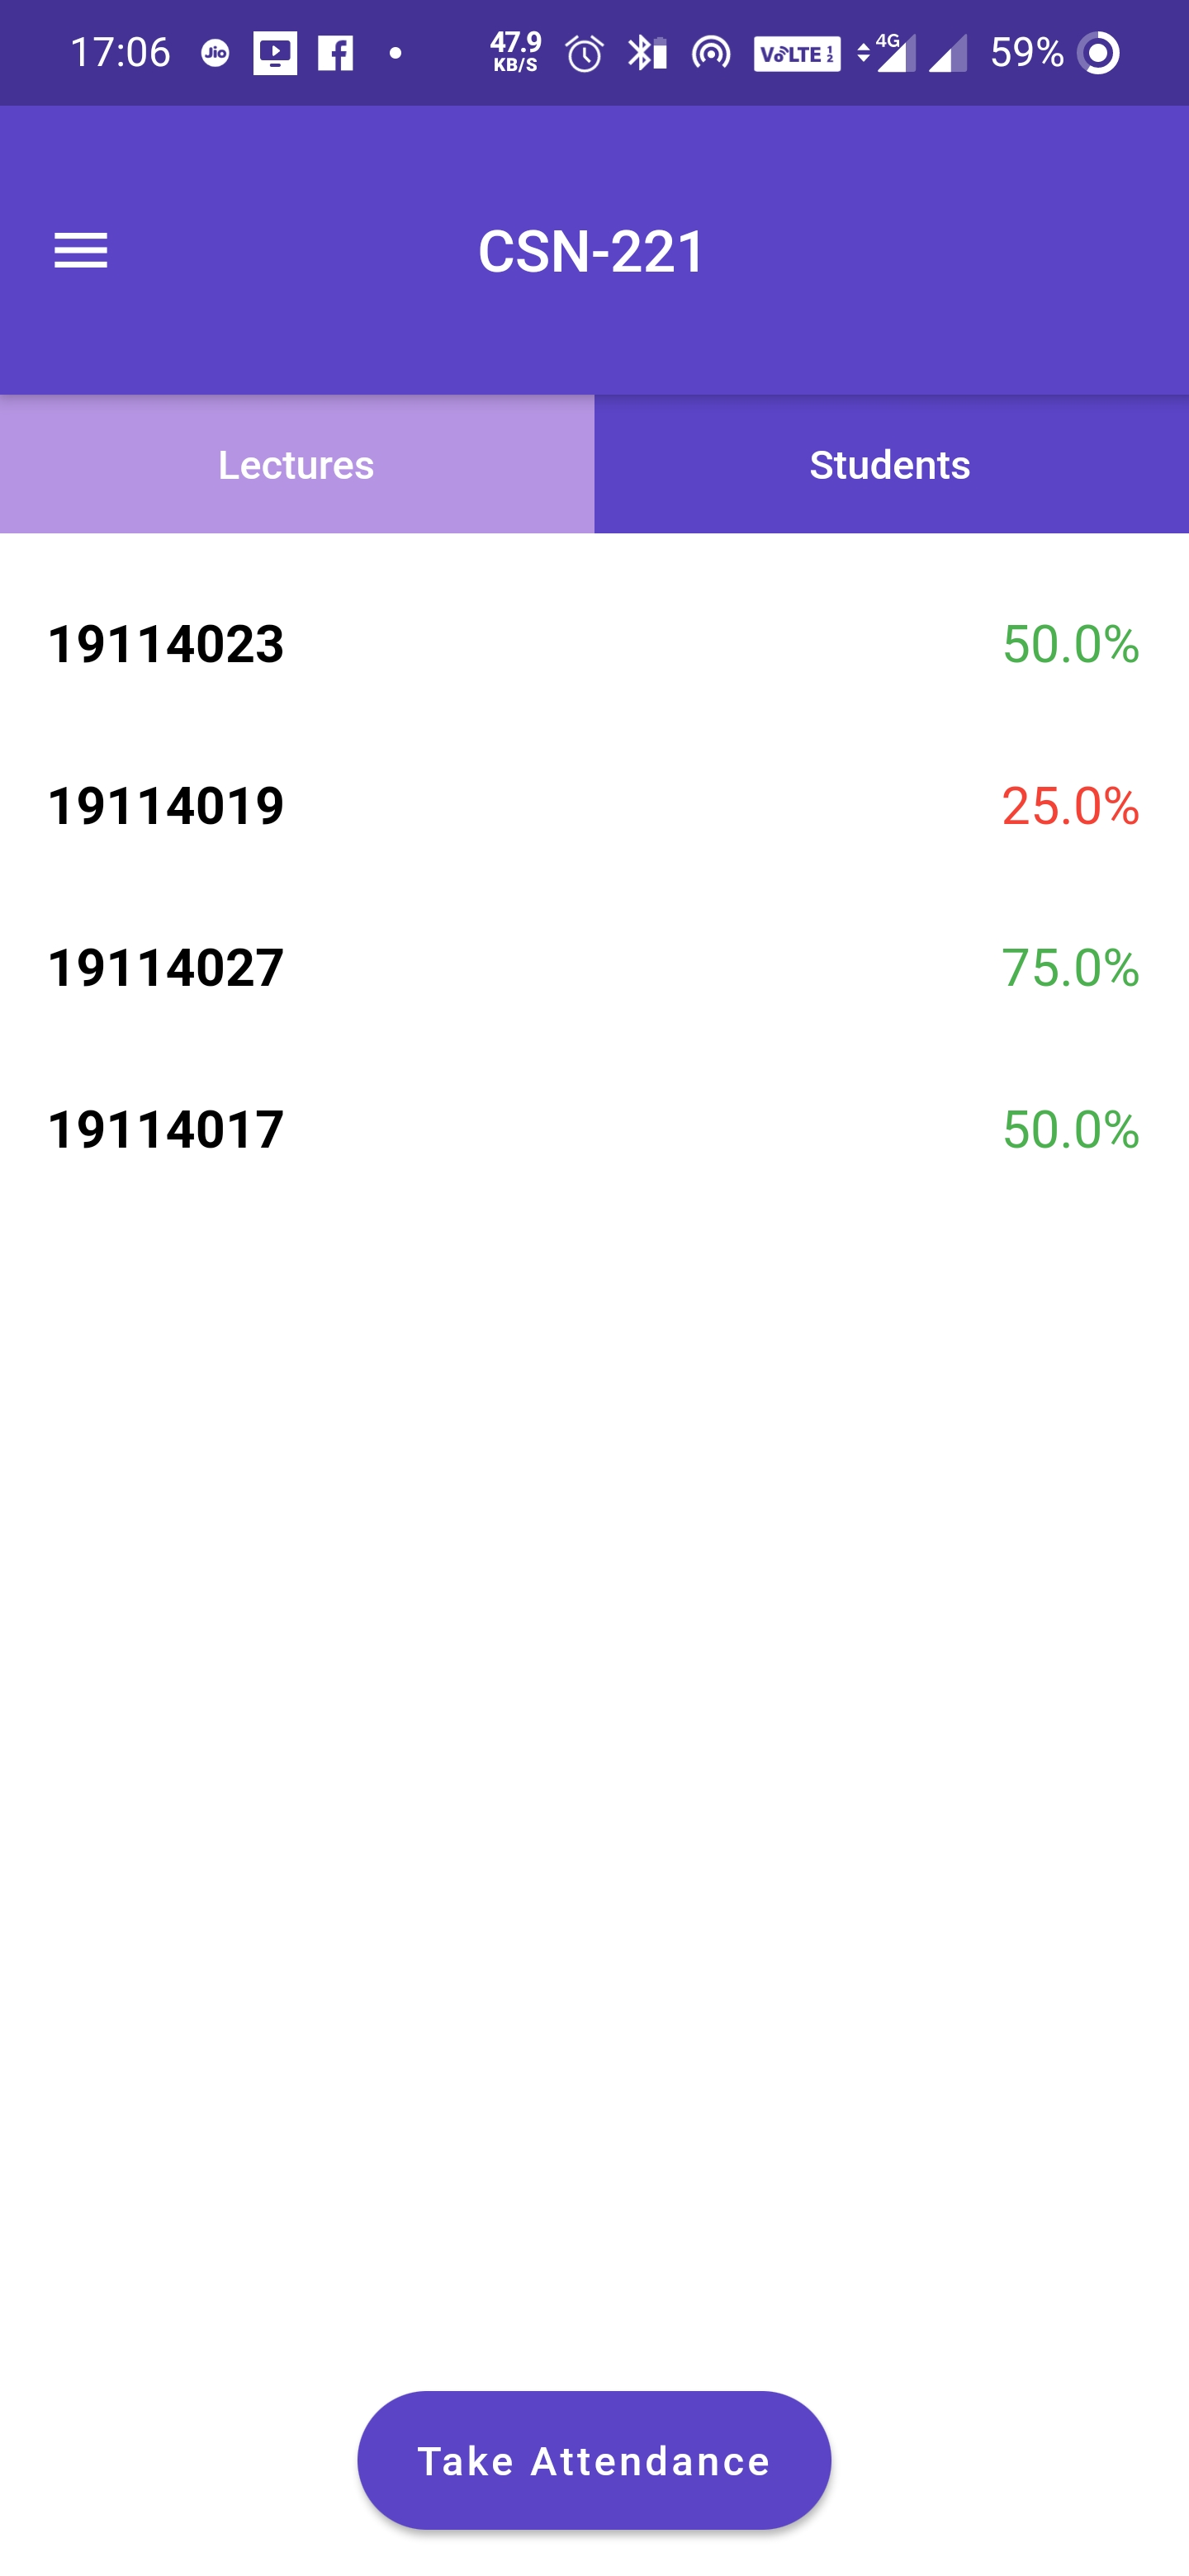
\includegraphics[width=0.40\textwidth]{Lectures.jpg}
    \caption{Lecture details and Student Stats}
    \label{fig:LecSt}
\end{figure}
\begin{figure}[H]
    \centering
    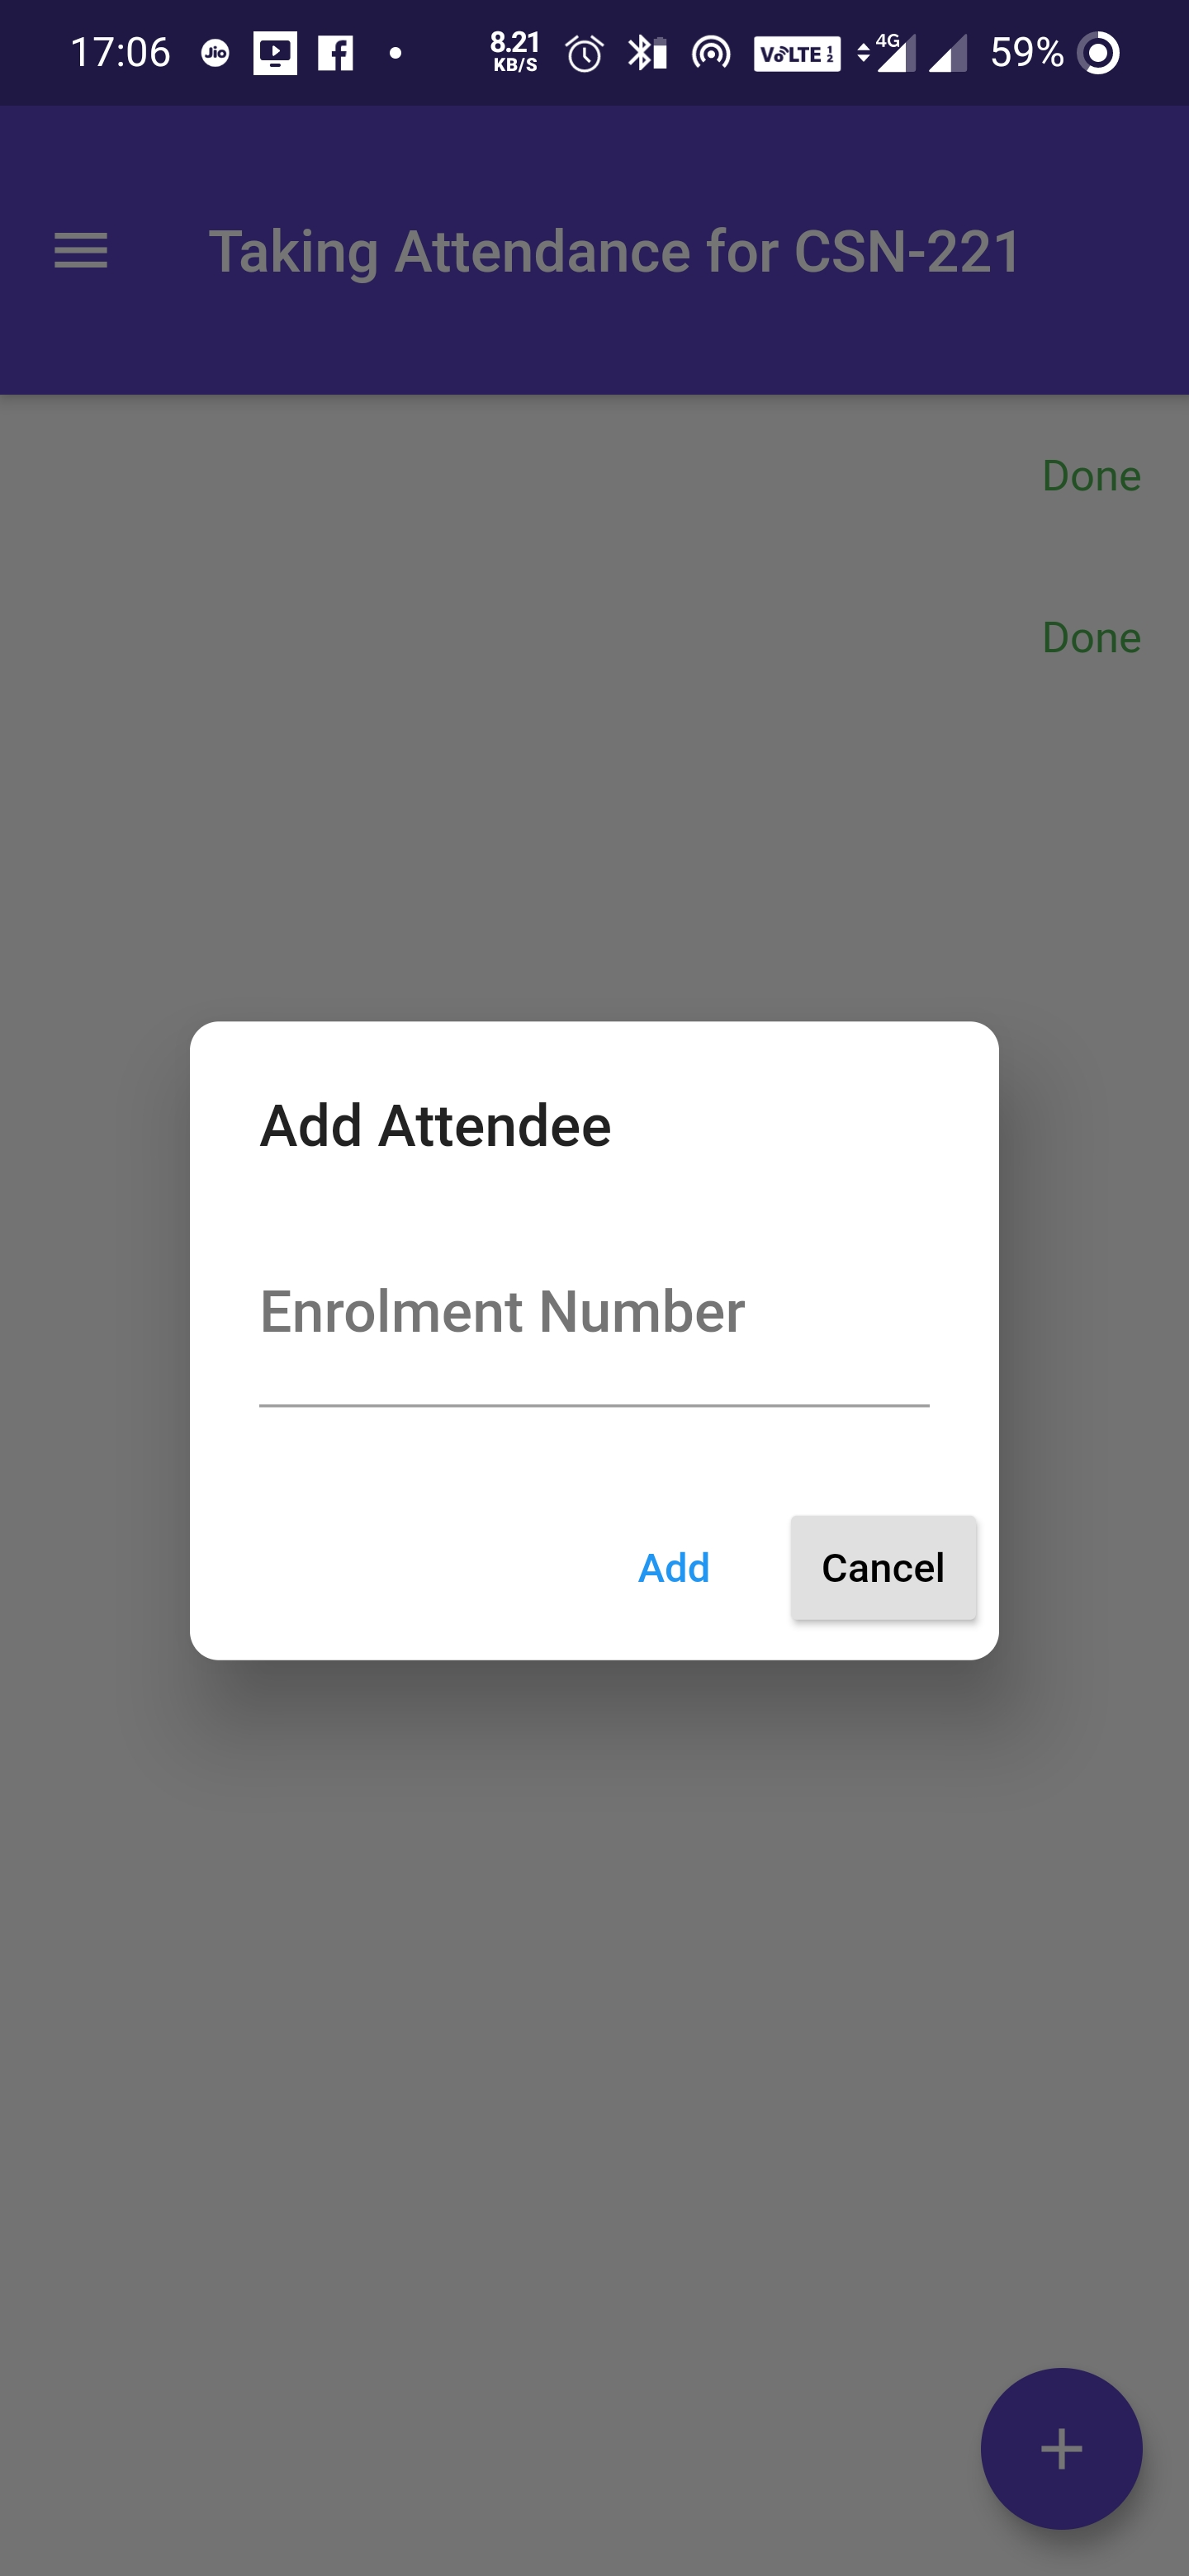
\includegraphics[width=0.50\textwidth]{AddAttendee.jpg}
    \caption{Add Student attendance manually}
    \label{fig:AddStudent}
\end{figure}
\section{References and tools}
Firebase related links :
\begin{enumerate}
    \item \url{https://firebase.google.com/docs}
    \item \url{https://www.youtube.com/watch?v=sfA3NWDBPZ4&list=PL4cUxeGkcC9j--TKIdkb3ISfRbJeJYQwC}
    \item \url{https://www.youtube.com/playlist?list=PLl-K7zZEsYLluG5MCVEzXAQ7ACZBCuZgZ}
    \item \url{https://medium.com/flutterdevs/using-firebase-firestore-in-flutter-b0ea2c62bc7}
\end{enumerate}
Networking related links :
\begin{enumerate}
    \item \url{https://jamesslocum.com/blog/post/67566023889}
    \item \url{https://developer.android.com/training/connect-devices-wirelessly/nsd#kotlin}
    \item \url{https://pub.dev/packages/bonsoir}
\end{enumerate}
Flutter related links :
\begin{enumerate}
    \item \url{https://flutter.dev/}
    \item \url{https://api.flutter.dev/flutter/dart-core/dart-core-library.html}
\end{enumerate}
    
\end{document}
